% Options for packages loaded elsewhere
% Options for packages loaded elsewhere
\PassOptionsToPackage{unicode}{hyperref}
\PassOptionsToPackage{hyphens}{url}
%
\documentclass[
  11pt,
  letterpaper,
]{book}
\usepackage{xcolor}
\usepackage[margin=2.5cm,paper=a4paper]{geometry}
\usepackage{amsmath,amssymb}
\setcounter{secnumdepth}{5}
\usepackage{iftex}
\ifPDFTeX
  \usepackage[T1]{fontenc}
  \usepackage[utf8]{inputenc}
  \usepackage{textcomp} % provide euro and other symbols
\else % if luatex or xetex
  \usepackage{unicode-math} % this also loads fontspec
  \defaultfontfeatures{Scale=MatchLowercase}
  \defaultfontfeatures[\rmfamily]{Ligatures=TeX,Scale=1}
\fi
\usepackage{lmodern}
\ifPDFTeX\else
  % xetex/luatex font selection
\fi
% Use upquote if available, for straight quotes in verbatim environments
\IfFileExists{upquote.sty}{\usepackage{upquote}}{}
\IfFileExists{microtype.sty}{% use microtype if available
  \usepackage[]{microtype}
  \UseMicrotypeSet[protrusion]{basicmath} % disable protrusion for tt fonts
}{}
\makeatletter
\@ifundefined{KOMAClassName}{% if non-KOMA class
  \IfFileExists{parskip.sty}{%
    \usepackage{parskip}
  }{% else
    \setlength{\parindent}{0pt}
    \setlength{\parskip}{6pt plus 2pt minus 1pt}}
}{% if KOMA class
  \KOMAoptions{parskip=half}}
\makeatother
% Make \paragraph and \subparagraph free-standing
\makeatletter
\ifx\paragraph\undefined\else
  \let\oldparagraph\paragraph
  \renewcommand{\paragraph}{
    \@ifstar
      \xxxParagraphStar
      \xxxParagraphNoStar
  }
  \newcommand{\xxxParagraphStar}[1]{\oldparagraph*{#1}\mbox{}}
  \newcommand{\xxxParagraphNoStar}[1]{\oldparagraph{#1}\mbox{}}
\fi
\ifx\subparagraph\undefined\else
  \let\oldsubparagraph\subparagraph
  \renewcommand{\subparagraph}{
    \@ifstar
      \xxxSubParagraphStar
      \xxxSubParagraphNoStar
  }
  \newcommand{\xxxSubParagraphStar}[1]{\oldsubparagraph*{#1}\mbox{}}
  \newcommand{\xxxSubParagraphNoStar}[1]{\oldsubparagraph{#1}\mbox{}}
\fi
\makeatother

\usepackage{color}
\usepackage{fancyvrb}
\newcommand{\VerbBar}{|}
\newcommand{\VERB}{\Verb[commandchars=\\\{\}]}
\DefineVerbatimEnvironment{Highlighting}{Verbatim}{commandchars=\\\{\}}
% Add ',fontsize=\small' for more characters per line
\usepackage{framed}
\definecolor{shadecolor}{RGB}{241,243,245}
\newenvironment{Shaded}{\begin{snugshade}}{\end{snugshade}}
\newcommand{\AlertTok}[1]{\textcolor[rgb]{0.68,0.00,0.00}{#1}}
\newcommand{\AnnotationTok}[1]{\textcolor[rgb]{0.37,0.37,0.37}{#1}}
\newcommand{\AttributeTok}[1]{\textcolor[rgb]{0.40,0.45,0.13}{#1}}
\newcommand{\BaseNTok}[1]{\textcolor[rgb]{0.68,0.00,0.00}{#1}}
\newcommand{\BuiltInTok}[1]{\textcolor[rgb]{0.00,0.23,0.31}{#1}}
\newcommand{\CharTok}[1]{\textcolor[rgb]{0.13,0.47,0.30}{#1}}
\newcommand{\CommentTok}[1]{\textcolor[rgb]{0.37,0.37,0.37}{#1}}
\newcommand{\CommentVarTok}[1]{\textcolor[rgb]{0.37,0.37,0.37}{\textit{#1}}}
\newcommand{\ConstantTok}[1]{\textcolor[rgb]{0.56,0.35,0.01}{#1}}
\newcommand{\ControlFlowTok}[1]{\textcolor[rgb]{0.00,0.23,0.31}{\textbf{#1}}}
\newcommand{\DataTypeTok}[1]{\textcolor[rgb]{0.68,0.00,0.00}{#1}}
\newcommand{\DecValTok}[1]{\textcolor[rgb]{0.68,0.00,0.00}{#1}}
\newcommand{\DocumentationTok}[1]{\textcolor[rgb]{0.37,0.37,0.37}{\textit{#1}}}
\newcommand{\ErrorTok}[1]{\textcolor[rgb]{0.68,0.00,0.00}{#1}}
\newcommand{\ExtensionTok}[1]{\textcolor[rgb]{0.00,0.23,0.31}{#1}}
\newcommand{\FloatTok}[1]{\textcolor[rgb]{0.68,0.00,0.00}{#1}}
\newcommand{\FunctionTok}[1]{\textcolor[rgb]{0.28,0.35,0.67}{#1}}
\newcommand{\ImportTok}[1]{\textcolor[rgb]{0.00,0.46,0.62}{#1}}
\newcommand{\InformationTok}[1]{\textcolor[rgb]{0.37,0.37,0.37}{#1}}
\newcommand{\KeywordTok}[1]{\textcolor[rgb]{0.00,0.23,0.31}{\textbf{#1}}}
\newcommand{\NormalTok}[1]{\textcolor[rgb]{0.00,0.23,0.31}{#1}}
\newcommand{\OperatorTok}[1]{\textcolor[rgb]{0.37,0.37,0.37}{#1}}
\newcommand{\OtherTok}[1]{\textcolor[rgb]{0.00,0.23,0.31}{#1}}
\newcommand{\PreprocessorTok}[1]{\textcolor[rgb]{0.68,0.00,0.00}{#1}}
\newcommand{\RegionMarkerTok}[1]{\textcolor[rgb]{0.00,0.23,0.31}{#1}}
\newcommand{\SpecialCharTok}[1]{\textcolor[rgb]{0.37,0.37,0.37}{#1}}
\newcommand{\SpecialStringTok}[1]{\textcolor[rgb]{0.13,0.47,0.30}{#1}}
\newcommand{\StringTok}[1]{\textcolor[rgb]{0.13,0.47,0.30}{#1}}
\newcommand{\VariableTok}[1]{\textcolor[rgb]{0.07,0.07,0.07}{#1}}
\newcommand{\VerbatimStringTok}[1]{\textcolor[rgb]{0.13,0.47,0.30}{#1}}
\newcommand{\WarningTok}[1]{\textcolor[rgb]{0.37,0.37,0.37}{\textit{#1}}}

\usepackage{longtable,booktabs,array}
\usepackage{calc} % for calculating minipage widths
% Correct order of tables after \paragraph or \subparagraph
\usepackage{etoolbox}
\makeatletter
\patchcmd\longtable{\par}{\if@noskipsec\mbox{}\fi\par}{}{}
\makeatother
% Allow footnotes in longtable head/foot
\IfFileExists{footnotehyper.sty}{\usepackage{footnotehyper}}{\usepackage{footnote}}
\makesavenoteenv{longtable}
\usepackage{graphicx}
\makeatletter
\newsavebox\pandoc@box
\newcommand*\pandocbounded[1]{% scales image to fit in text height/width
  \sbox\pandoc@box{#1}%
  \Gscale@div\@tempa{\textheight}{\dimexpr\ht\pandoc@box+\dp\pandoc@box\relax}%
  \Gscale@div\@tempb{\linewidth}{\wd\pandoc@box}%
  \ifdim\@tempb\p@<\@tempa\p@\let\@tempa\@tempb\fi% select the smaller of both
  \ifdim\@tempa\p@<\p@\scalebox{\@tempa}{\usebox\pandoc@box}%
  \else\usebox{\pandoc@box}%
  \fi%
}
% Set default figure placement to htbp
\def\fps@figure{htbp}
\makeatother

\ifLuaTeX
  \usepackage{luacolor}
  \usepackage[soul]{lua-ul}
\else
  \usepackage{soul}
\fi




\setlength{\emergencystretch}{3em} % prevent overfull lines

\providecommand{\tightlist}{%
  \setlength{\itemsep}{0pt}\setlength{\parskip}{0pt}}



 
\usepackage[]{biblatex}
\addbibresource{ref/MAref.bib}


% AMTAIR Thesis Preamble - Zero package conflicts
% Only formatting commands, no package loading

% Line spacing for academic work
\usepackage{setspace}
\onehalfspacing

% Custom chapter formatting (remove "Chapter N" prefix) but unfortunately leaves blank space
\usepackage{titlesec}
\titleformat{\chapter}[display]
  {\normalfont\huge\bfseries}  % format
  {}                           % label (empty = no "Chapter N")
  {0pt}                        % sep
  {\Huge}                      % before-code



% Page formatting and headers
\usepackage{fancyhdr}
\pagestyle{fancy}
\fancyhf{}
\fancyhead[LE,RO]{\slshape\nouppercase{\rightmark}}
\fancyhead[LO,RE]{\slshape\nouppercase{\leftmark}}
\fancyfoot[C]{\thepage}

% % Fix page breaks after title page
% \newcommand{\cleartitlepage}{
%   \clearpage
%   \thispagestyle{empty}
%   \mbox{}
%   \clearpage
% }



\renewcommand{\maketitle}{}

%  Citation customization
% \usepackage[style=authoryear,backend=biber,natbib=true]{biblatex}

% % Custom citation commands for different contexts
% \newcommand{\citeauthor}[1]{\textcite{#1}}           % Author (year)
% \newcommand{\citeyear}[1]{(\citeyear*{#1})}         % (year)
% \newcommand{\citealt}[1]{\citeauthor{#1} \citeyear{#1}}  % Author year
% \newcommand{\citep}[1]{(\cite{#1})}                 # (Author, year)

% Page reference styling
% \DeclareFieldFormat{postnote}{#1}                    # No "p." prefix
% \DeclareFieldFormat{multipostnote}{#1}               # No "pp." prefix


% % Page numbering control
% \usepackage{afterpage}

% % Command to start front matter (roman numerals)
% \newcommand{\frontmatter}{
%   \cleardoublepage
%   \pagenumbering{roman}
%   \setcounter{page}{1}
% }

% % Command to start main matter (arabic numerals)
% \newcommand{\mainmatter}{
%   \cleardoublepage
%   \pagenumbering{arabic}
%   \setcounter{page}{1}
% }

% % Command to start back matter (continue arabic)
% \newcommand{\backmatter}{
%   \cleardoublepage
%   % Keep arabic numbering but could change style if needed
% }

% % Suppress page numbers on title page
% \newcommand{\titlepage}{
%   \thispagestyle{empty}
% }



% Commands for custom title page
% \newcommand{\thesistitle}{Automating the Modelling of Transformative Artificial Intelligence Risks}
% \newcommand{\thesisauthor}{Valentin Jakob Meyer}
\makeatletter
\@ifpackageloaded{tcolorbox}{}{\usepackage[skins,breakable]{tcolorbox}}
\@ifpackageloaded{fontawesome5}{}{\usepackage{fontawesome5}}
\definecolor{quarto-callout-color}{HTML}{909090}
\definecolor{quarto-callout-note-color}{HTML}{0758E5}
\definecolor{quarto-callout-important-color}{HTML}{CC1914}
\definecolor{quarto-callout-warning-color}{HTML}{EB9113}
\definecolor{quarto-callout-tip-color}{HTML}{00A047}
\definecolor{quarto-callout-caution-color}{HTML}{FC5300}
\definecolor{quarto-callout-color-frame}{HTML}{acacac}
\definecolor{quarto-callout-note-color-frame}{HTML}{4582ec}
\definecolor{quarto-callout-important-color-frame}{HTML}{d9534f}
\definecolor{quarto-callout-warning-color-frame}{HTML}{f0ad4e}
\definecolor{quarto-callout-tip-color-frame}{HTML}{02b875}
\definecolor{quarto-callout-caution-color-frame}{HTML}{fd7e14}
\makeatother
\makeatletter
\@ifpackageloaded{bookmark}{}{\usepackage{bookmark}}
\makeatother
\makeatletter
\@ifpackageloaded{caption}{}{\usepackage{caption}}
\AtBeginDocument{%
\ifdefined\contentsname
  \renewcommand*\contentsname{Table of contents}
\else
  \newcommand\contentsname{Table of contents}
\fi
\ifdefined\listfigurename
  \renewcommand*\listfigurename{List of Figures}
\else
  \newcommand\listfigurename{List of Figures}
\fi
\ifdefined\listtablename
  \renewcommand*\listtablename{List of Tables}
\else
  \newcommand\listtablename{List of Tables}
\fi
\ifdefined\figurename
  \renewcommand*\figurename{Figure}
\else
  \newcommand\figurename{Figure}
\fi
\ifdefined\tablename
  \renewcommand*\tablename{Table}
\else
  \newcommand\tablename{Table}
\fi
}
\@ifpackageloaded{float}{}{\usepackage{float}}
\floatstyle{ruled}
\@ifundefined{c@chapter}{\newfloat{codelisting}{h}{lop}}{\newfloat{codelisting}{h}{lop}[chapter]}
\floatname{codelisting}{Listing}
\newcommand*\listoflistings{\listof{codelisting}{List of Listings}}
\makeatother
\makeatletter
\usepackage{pdflscape}
\makeatother
\makeatletter
\makeatother
\makeatletter
\@ifpackageloaded{caption}{}{\usepackage{caption}}
\@ifpackageloaded{subcaption}{}{\usepackage{subcaption}}
\makeatother
\usepackage{bookmark}
\IfFileExists{xurl.sty}{\usepackage{xurl}}{} % add URL line breaks if available
\urlstyle{same}
\hypersetup{
  pdftitle={Automating the Modelling of Transformative Artificial Intelligence Risks},
  pdfauthor={Valentin Jakob Meyer},
  hidelinks,
  pdfcreator={LaTeX via pandoc}}


\title{Automating the Modelling of Transformative Artificial
Intelligence Risks}
\usepackage{etoolbox}
\makeatletter
\providecommand{\subtitle}[1]{% add subtitle to \maketitle
  \apptocmd{\@title}{\par {\large #1 \par}}{}{}
}
\makeatother
\subtitle{An Epistemic Framework for Leveraging Frontier AI Systems to
Upscale Conditional Policy Assessments in Bayesian Networks on a Narrow
Path towards Existential Safety}
\author{Valentin Jakob Meyer}
\date{2025-05-26}
\begin{document}
\frontmatter
\maketitle

\begin{titlepage}
\thispagestyle{empty}% Remove page number from title page

% Top header with logo (left) and department (right)
\begin{minipage}{0.3\textwidth}
  
\includegraphics[width=5cm]{latex/uni-bayreuth-logo.png}
\end{minipage}
\hfill
\begin{minipage}{0.9\textwidth}
  \begin{center}
    -- P\&E Master's Programme --\\
    Chair of Philosophy, Computer\\
    Science \& Artificial Intelligence
  \end{center}
\end{minipage}

% Horizontal rule
\vspace{1.5cm}
\hrule
\vspace{2cm}

% Title in bold
\begin{center}
  \Large\textbf{Automating the Modelling of
Transformative Artificial Intelligence Risks}
\end{center}
\vspace{0.2cm}

\begin{center}
  -----
\end{center}
\vspace{0.2cm}

% Subtitle in italics with quotation marks
\begin{center}
  \normalsize``\textit{An Epistemic Framework for Leveraging Frontier AI Systems
to Upscale Conditional Policy Assessments in Bayesian Networks on a Narrow Path towards Existencial Safety }''
\end{center}
\vspace{0.2cm}

\begin{center}
  -----
\end{center}
\vspace{0.2cm}

% Thesis designation
\begin{center}
  A thesis submitted at the Department of Philosophy\\[0.4cm]
  for the degree of \textit{Master of Arts in Philosophy \& Economics}
\end{center}

\vspace{1.5cm}
% Horizontal rule
\hrule
\vspace{1.5cm}

% Author and supervisor information with precise alignment
\begin{minipage}[t]{0.48\textwidth}
  \textbf{Author:}\\[0.3cm]
  \href{https://www.vjmeyer.org}{Valentin Jakob Meyer}\\
  \href{mailto:Valentin.meyer@uni-bayreuth.de}{Valentin.meyer@uni-bayreuth.de}\\
  \textit{Matriculation Number:} 1828610\\
  \textit{Tel.:} +49 (1573) 4512494\\
  Pielmühler Straße 15\\
  52066 Lappersdorf
\end{minipage}
\hfill
\begin{minipage}[t]{0.48\textwidth}
  \begin{flushright}
    \textbf{Supervisor:}\\[0.3cm]
    \href{mailto:timo.speith@uni-bayreuth.de}{Dr. Timo Speith}\\[0.35cm]
    \textit{Word Count:}\\
    30.000\\[0.1cm]
    \textit{Source / Identifier:}\\
    \href{https://github.com/VJMeyer/submission}{Document URL}
  \end{flushright}
\end{minipage}

% Date at bottom
\vfill
\begin{center}
  26th of May 2025
\end{center}
\end{titlepage}

% Critical: Clean page break to TOC
\cleardoublepage

\renewcommand*\contentsname{Table of Contents}
{
\setcounter{tocdepth}{2}
\tableofcontents
}
\listoffigures
\listoftables

\mainmatter
\bookmarksetup{startatroot}

\chapter*{Preface}\label{preface}
\addcontentsline{toc}{chapter}{Preface}

\markboth{Preface}{Preface}

\bookmarksetup{startatroot}

\chapter*{Quarto Syntax}\label{sec-syntax}
\addcontentsline{toc}{chapter}{Quarto Syntax}

\markboth{Quarto Syntax}{Quarto Syntax}

\section*{Main Formatting}\label{main-formatting}
\addcontentsline{toc}{section}{Main Formatting}

\markright{Main Formatting}

\subsection*{Html Comments}\label{html-comments}
\addcontentsline{toc}{subsection}{Html Comments}

\section*{Syntax for Tasks}\label{syntax-for-tasks}
\addcontentsline{toc}{section}{Syntax for Tasks}

\markright{Syntax for Tasks}

\subsection*{Tasks with ToDo Tree}\label{tasks-with-todo-tree}
\addcontentsline{toc}{subsection}{Tasks with ToDo Tree}

\subsubsection*{Simple ``One-line tasks''}\label{simple-one-line-tasks}
\addcontentsline{toc}{subsubsection}{Simple ``One-line tasks''}

Use Code ticks and html comment and task format for tasks distinctly
visible across all formats including the ToDo-Tree overview:

\texttt{\textless{}!-\/-\ {[}\ {]}\ ToDos\ for\ things\ to\ do\ /\ tasks\ /\ reminders\ (allows\ "jump\ to\ with\ Taks\ Tree\ extension")\ -\/-\textgreater{}}

Use html comment and task format for open or uncertain tasks, visible in
the .qmd file:

\subsubsection*{More Complex Tasks with
Notes}\label{more-complex-tasks-with-notes}
\addcontentsline{toc}{subsubsection}{More Complex Tasks with Notes}

\begin{verbatim}
<!-- [ ] Task Title: short description-->

  More Information about task

  Relevant notes

  Step-by-step implementation Plan

  Etc.
\end{verbatim}

\subsubsection*{Completed Tasks}\label{completed-tasks}
\addcontentsline{toc}{subsubsection}{Completed Tasks}

Retain completed tasks in ToDo-Tree by adding an x in the brackets:
\texttt{{[}x{]}}
\texttt{\textless{}!-\/-\ {[}x{]}\ Tasks\ which\ have\ been\ finished\ but\ should\ remain\ for\ later\ verification\ -\/-\textgreater{}}

Mark and remove completed tasks from ToDo-Tree by adding a minus in the
brackets: \texttt{{[}-{]}}

\texttt{\textless{}!-\/-\ {[}-{]}\ Tasks\ which\ have\ been\ finished\ but\ should\ remain\ visible\ for\ later\ verification\ -\/-\textgreater{}}

\subsubsection*{Missing Citations}\label{missing-citations}
\addcontentsline{toc}{subsubsection}{Missing Citations}

\texttt{\textless{}!-\/-\ {[}\ {]}\ FIND:\ @CITATION\_KEY\_PURPOSE:\ "Description\ of\ the\ appropriate/idea\ source,\ including\ ideas\ /suggestions\ /\ search\ terms\ etc."\ -\/-\textgreater{}}

\subsubsection*{Suggested Citation}\label{suggested-citation}
\addcontentsline{toc}{subsubsection}{Suggested Citation}

\texttt{\textless{}!-\/-\ {[}\ {]}\ VERIFY:\ @CITATION\_KEY\_SUGGESTED:\ "Description\ of\ the\ appropriate\ paper,\ book,\ source"\ {[}Include\ BibTex\ if\ known{]}\ -\/-\textgreater{}}

\subsubsection*{Missing Graphic}\label{missing-graphic}
\addcontentsline{toc}{subsubsection}{Missing Graphic}

\texttt{\textless{}!-\/-\ {[}\ {]}\ FIND:\ \{\#fig-GRAPHIC\_IDEA\}{]}:\ "Description\ of\ the\ appropriate/idea\ source,\ including\ ideas\ /suggestions\ /\ search\ terms\ etc."\ -\/-\textgreater{}}

\subsubsection*{Suggested Graphic}\label{suggested-graphic}
\addcontentsline{toc}{subsubsection}{Suggested Graphic}

\texttt{\textless{}!-\/-\ {[}\ {]}\ VERIFY:\ \{\#fig-GRAPHIC\_IDEA\}:\ "Description\ of\ the\ appropriate\ paper,\ book,\ source"\ {[}Include\ figure\ syntax\ if\ known{]}\ -\/-\textgreater{}}

Missing and/or suggested tables, concepts, explanations as well as other
elements should be suggested similarily.

\subsection*{Task Syntax Examples}\label{task-syntax-examples}
\addcontentsline{toc}{subsection}{Task Syntax Examples}

\texttt{\textless{}!-\/-\ {[}\ {]}\ (Example\ short:\ open\ and\ visible\ in\ text)\ \ \ Find\ and\ list\ the\ names\ of\ the\ MTAIR\ team-members\ responsible\ for\ the\ Analytica\ Implementation\ -\/-\textgreater{}}

\begin{verbatim}
<!-- [ ] (Example longer: open and visible in text)    Review/Plan/Discuss integrating Live Prediction Markets -->

  Live prediction market integration requires:
    (1) API connections to platforms (Metaculus, Manifold),
    (2) Question-to-variable mapping algorithms,
    (3) Probability update mechanisms, 
    (4) Handling of market dynamics (thin markets, manipulation).
    Current mentions may overstate readiness or underestimate complexity.
    Need realistic assessment of what's achievable.

  Implementation Steps:
      0. List/mention all relevant platforms with a brief description each
      1. Review all existing prediction market mentions for accuracy
      2. Assess actual API availability and limitations
      3. Describe/explain/discuss how to implement basic proof-of-concept with single platform
      4. Document challenges: question mapping, market interpretation
      5. Create realistic timeline for full implementation
      6. Revise thesis claims to match reality
      7. Add "Future Work" and/or extension section on complete integration
      8. Include descriptions of mockups/designs even if not fully built 
      9. Highlight/discuss the advantages of such integrations
      10. Quickly brainstorm for downsides worth mentioning
\end{verbatim}

\subsection*{Verbatim Code Formatting}\label{verbatim-code-formatting}
\addcontentsline{toc}{subsection}{Verbatim Code Formatting}

\texttt{verbatim\ code\ formatting\ for\ notes\ and\ ideas\ to\ be\ included\ (here)}

\subsection*{Code Block formatting}\label{code-block-formatting}
\addcontentsline{toc}{subsection}{Code Block formatting}

\begin{verbatim}
Also code blocks for more extensive notes and ideas to be included and checklists
- test 1. 
- test 2. 
- test 3.
2. second
3. third
\end{verbatim}

\begin{verbatim}
code
\end{verbatim}

Add a language to syntax highlight code blocks:

\begin{Shaded}
\begin{Highlighting}[]
\DecValTok{1} \OperatorTok{+} \DecValTok{1}
\end{Highlighting}
\end{Shaded}

\subsection*{Blockquote Formatting}\label{blockquote-formatting}
\addcontentsline{toc}{subsection}{Blockquote Formatting}

\begin{quote}
Blockquote formatting for ``Suggested Citations (e.g.~carlsmith 2024 on
\ldots)'' and/or claims which require a citation (e.g.~claim x should be
backed-up by a ciation from the literature)
\end{quote}

\subsection*{Tables}\label{tables}
\addcontentsline{toc}{subsection}{Tables}

\begin{longtable}[]{@{}rllc@{}}
\caption{Demonstration of pipe table
syntax}\label{tbl-letters}\tabularnewline
\toprule\noalign{}
Right & Left & Default & Center \\
\midrule\noalign{}
\endfirsthead
\toprule\noalign{}
Right & Left & Default & Center \\
\midrule\noalign{}
\endhead
\bottomrule\noalign{}
\endlastfoot
12 & 12 & 12 & 12 \\
123 & 123 & 123 & 123 \\
1 & 1 & 1 & 1 \\
\end{longtable}

\begin{longtable}[]{@{}lll@{}}
\caption{My Caption 1}\label{tbl-letters}\tabularnewline
\toprule\noalign{}
Col1 & Col2 & Col3 \\
\midrule\noalign{}
\endfirsthead
\toprule\noalign{}
Col1 & Col2 & Col3 \\
\midrule\noalign{}
\endhead
\bottomrule\noalign{}
\endlastfoot
A & B & C \\
E & F & G \\
A & G & G \\
\end{longtable}

Referencing tables with \texttt{@tbl-KEY}: See Table~\ref{tbl-letters}.

\begin{table}

\caption{\label{tbl-panel}Main Caption}

\begin{minipage}{0.50\linewidth}

\subcaption{\label{tbl-first}First Table}

\centering{

\begin{tabular}{lll}
\toprule
Col1 & Col2 & Col3\\
\midrule
A & B & C\\
E & F & G\\
A & G & G\\
\bottomrule
\end{tabular}

}

\end{minipage}%
%
\begin{minipage}{0.50\linewidth}

\subcaption{\label{tbl-second}Second Table}

\centering{

\begin{tabular}{lll}
\toprule
Col1 & Col2 & Col3\\
\midrule
A & B & C\\
E & F & G\\
A & G & G\\
\bottomrule
\end{tabular}

}

\end{minipage}%

\end{table}%

See Table~\ref{tbl-panel} for details, especially
Table~\ref{tbl-second}.

\begin{Shaded}
\begin{Highlighting}[]
\NormalTok{python}
\NormalTok{\#| label: tbl{-}planets}
\NormalTok{\#| tbl{-}cap: Astronomical object}

\NormalTok{from IPython.display import Markdown}
\NormalTok{from tabulate import tabulate}
\NormalTok{table = [}\CommentTok{[}\OtherTok{"Sun","696,000",1.989e30}\CommentTok{]}\NormalTok{,}
         \CommentTok{[}\OtherTok{"Earth","6,371",5.972e24}\CommentTok{]}\NormalTok{,}
         \CommentTok{[}\OtherTok{"Moon","1,737",7.34e22}\CommentTok{]}\NormalTok{,}
         \CommentTok{[}\OtherTok{"Mars","3,390",6.39e23}\CommentTok{]}\NormalTok{]}
\NormalTok{Markdown(tabulate(}
\NormalTok{  table, }
\NormalTok{  headers=}\CommentTok{[}\OtherTok{"Astronomical object","R (km)", "mass (kg)"}\CommentTok{]}
\NormalTok{))}
\end{Highlighting}
\end{Shaded}

\begin{longtable}[]{@{}
  >{\raggedright\arraybackslash}p{(\linewidth - 4\tabcolsep) * \real{0.1806}}
  >{\raggedright\arraybackslash}p{(\linewidth - 4\tabcolsep) * \real{0.1806}}
  >{\raggedright\arraybackslash}p{(\linewidth - 4\tabcolsep) * \real{0.3194}}@{}}
\caption{Sample grid table.}\tabularnewline
\toprule\noalign{}
\begin{minipage}[b]{\linewidth}\raggedright
Fruit
\end{minipage} & \begin{minipage}[b]{\linewidth}\raggedright
Price
\end{minipage} & \begin{minipage}[b]{\linewidth}\raggedright
Advantages
\end{minipage} \\
\midrule\noalign{}
\endfirsthead
\toprule\noalign{}
\begin{minipage}[b]{\linewidth}\raggedright
Fruit
\end{minipage} & \begin{minipage}[b]{\linewidth}\raggedright
Price
\end{minipage} & \begin{minipage}[b]{\linewidth}\raggedright
Advantages
\end{minipage} \\
\midrule\noalign{}
\endhead
\bottomrule\noalign{}
\endlastfoot
Bananas & \$1.34 & \begin{minipage}[t]{\linewidth}\raggedright
\begin{itemize}
\tightlist
\item
  built-in wrapper
\item
  bright color
\end{itemize}
\end{minipage} \\
Oranges & \$2.10 & \begin{minipage}[t]{\linewidth}\raggedright
\begin{itemize}
\tightlist
\item
  cures scurvy
\item
  tasty
\end{itemize}
\end{minipage} \\
\end{longtable}

Content with HTML tables you don't want processed.

\section*{Headings \& Potential Headings in Standard Markdown formatting
(`\#\#')}\label{sec-heading}
\addcontentsline{toc}{section}{Headings \& Potential Headings in
Standard Markdown formatting (`\#\#')}

\markright{Headings \& Potential Headings in Standard Markdown
formatting (`\#\#')}

\subsection*{Heading 3}\label{heading-3}
\addcontentsline{toc}{subsection}{Heading 3}

\subsubsection*{Heading 4}\label{heading-4}
\addcontentsline{toc}{subsubsection}{Heading 4}

\section*{Text Formatting Options}\label{text-formatting-options}
\addcontentsline{toc}{section}{Text Formatting Options}

\markright{Text Formatting Options}

\emph{italics}, \textbf{bold}, \textbf{\emph{bold italics}}

superscript\textsuperscript{2} and subscript\textsubscript{2}

\st{strikethrough}

\hl{This text is highlighted}

\ul{This text is underlined}

\textsc{This text is smallcaps}

\section*{Lists}\label{lists}
\addcontentsline{toc}{section}{Lists}

\markright{Lists}

\begin{itemize}
\item
  unordered list

  \begin{itemize}
  \tightlist
  \item
    sub-item 1
  \item
    sub-item 2

    \begin{itemize}
    \tightlist
    \item
      sub-sub-item 1
    \end{itemize}
  \end{itemize}
\item
  item 2

  Continued (indent 4 spaces)
\end{itemize}

\begin{enumerate}
\def\labelenumi{\arabic{enumi}.}
\tightlist
\item
  ordered list
\item
  item 2

  \begin{enumerate}
  \def\labelenumii{\roman{enumii})}
  \tightlist
  \item
    sub-item 1

    \begin{enumerate}
    \def\labelenumiii{\Alph{enumiii}.}
    \tightlist
    \item
      sub-sub-item 1
    \end{enumerate}
  \end{enumerate}
\end{enumerate}

\section*{Math}\label{math}
\addcontentsline{toc}{section}{Math}

\markright{Math}

inline math: \(E = mc^{2}\)

display math:

\[E = mc^{2}\]

If you want to define custom TeX macros, include them within \$\$
delimiters enclosed in a .hidden block. For example:

\[
 \def\RR{{\bf R}}
 \def\bold#1{{\bf #1}}
\]

For HTML math processed using MathJax (the default) you can use the
\textbackslash def, \textbackslash newcommand,
\textbackslash renewcommand, \textbackslash newenvironment,
\textbackslash renewenvironment, and \textbackslash let commands to
create your own macros and environments.

\section*{Footnotes}\label{footnotes}
\addcontentsline{toc}{section}{Footnotes}

\markright{Footnotes}

Here is an inline note.\footnote{Inlines notes are easier to write,
  since you don't have to pick an identifier and move down to type the
  note.}

Here is a footnote reference,\footnote{Here is the footnote.}

Another Text with a footnote\footnote{Here's one with multiple blocks.}
but this time a ``longnote''.

This paragraph won't be part of the note, because it isn't indented.

\section*{Callouts}\label{sec-callouts}
\addcontentsline{toc}{section}{Callouts}

\markright{Callouts}

Quarto's native callouts work without additional packages:

This is written in a `note' environment -- but it does not seem to
produce any special rendering.

\begin{tcolorbox}[enhanced jigsaw, coltitle=black, opacitybacktitle=0.6, titlerule=0mm, colframe=quarto-callout-note-color-frame, breakable, leftrule=.75mm, colback=white, left=2mm, opacityback=0, colbacktitle=quarto-callout-note-color!10!white, bottomtitle=1mm, toptitle=1mm, title=\textcolor{quarto-callout-note-color}{\faInfo}\hspace{0.5em}{Optional Title}, arc=.35mm, bottomrule=.15mm, rightrule=.15mm, toprule=.15mm]

Content here

\end{tcolorbox}

\begin{tcolorbox}[enhanced jigsaw, coltitle=black, opacitybacktitle=0.6, titlerule=0mm, colframe=quarto-callout-note-color-frame, breakable, leftrule=.75mm, colback=white, left=2mm, opacityback=0, colbacktitle=quarto-callout-note-color!10!white, bottomtitle=1mm, toptitle=1mm, title=\textcolor{quarto-callout-note-color}{\faInfo}\hspace{0.5em}{Important Note2}, arc=.35mm, bottomrule=.15mm, rightrule=.15mm, toprule=.15mm]

This renders perfectly in both HTML and PDF.

\end{tcolorbox}

Also for markdown:

\begin{Shaded}
\begin{Highlighting}[]
\NormalTok{::: \{.render\_as\_markdown\_example\}}
\FunctionTok{\#\# Markdown Heading}
\NormalTok{This renders perfectly in both HTML and PDF but as markdown "plain text"}
\NormalTok{:::}
\end{Highlighting}
\end{Shaded}

\section*{Links}\label{links}
\addcontentsline{toc}{section}{Links}

\markright{Links}

\texttt{\textless{}https://quarto.org/docs/authoring/markdown-basics.html\textgreater{}}
produces: \url{https://quarto.org/docs/authoring/markdown-basics.html}

\texttt{{[}Quarto\ Book\ Cross-References{]}(https://quarto.org/docs/books/book-crossrefs.html)}
produces:
\href{https://quarto.org/docs/books/book-crossrefs.html}{Quarto Book
Cross-References}

\section*{Images \& Figures}\label{sec-figures1}

\markright{Images \& Figures}

\begin{verbatim}
[![AMTAIR Automation Pipeline from @bucknall2022](/images/pipeline.png){
  #fig-automation_pipeline
  fig-scap="Five-step AMTAIR automation pipeline from PDFs to Bayesian networks" 
  fig-alt="FLOWCHART: Five-step automation pipeline workflow for AMTAIR project.
          DATA: The pipeline transforms PDFs through ArgDown, BayesDown, CSV, and HTML into Bayesian network visualizations.
          PURPOSE: Illustrates the core technical process that enables automated extraction of probabilistic models from AI safety literature.
          DETAILS: Five numbered green steps show: (1) LLM-based extraction from PDFs to ArgDown, (2) ArgDown to BayesDown completion with probabilities, (3) Extracting world-models as CSV data, (4) Software tools for data inference, and (5) Visualization of the resulting Bayesian network.
          Each step includes example outputs, with the final visualization showing a Rain-Sprinkler-Grass Wet Bayesian network with probability tables.
          SOURCE: Created by the author to explain the AMTAIR methodology
          "
  fig-align="center" 
  width="100%"
  }](https://github.com/VJMeyer/submission)


Testing crossreferencing grapics @fig-automation_pipeline.

![Caption/Title 2](/images/cover.png){#fig-testgraphic2 fig-scap="Short 2 caption" fig-alt="2nd Alt Text / Description." fig-align="left" width="30%"}

Testing crossreferencing grapics @fig-testgraphic2.
\end{verbatim}

\begin{figure}

\centering{

\href{https://github.com/VJMeyer/submission}{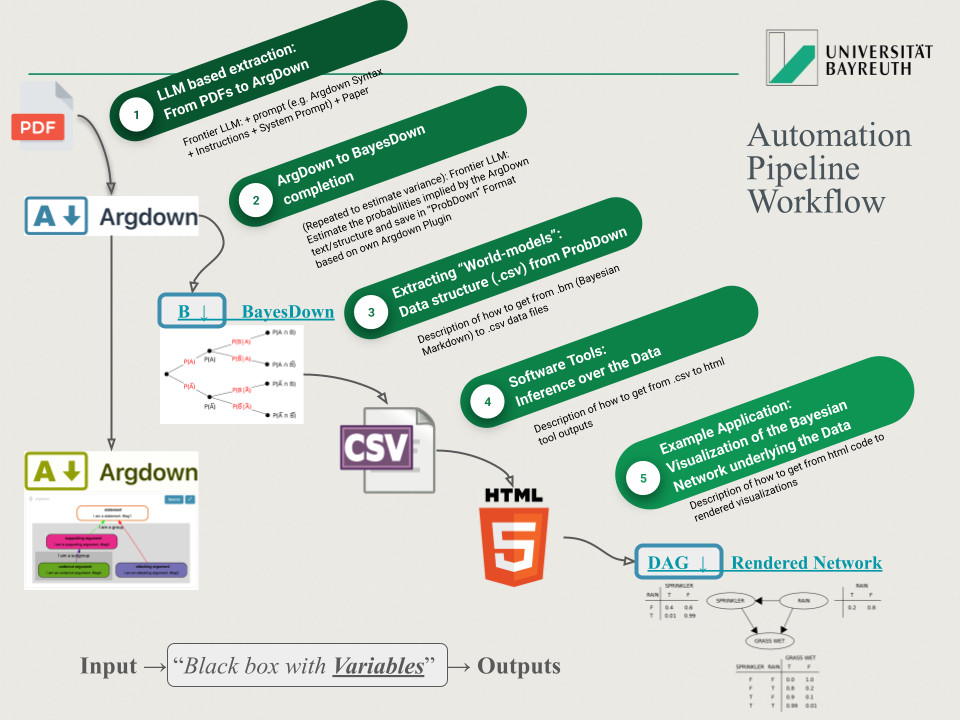
\includegraphics[width=1\linewidth,height=\textheight,keepaspectratio]{images/pipeline.png}}

}

\caption[Five-step AMTAIR automation pipeline from PDFs to Bayesian
networks]{\label{fig-automation_pipeline}AMTAIR Automation Pipeline
from}

\end{figure}%

Testing crossreferencing grapics Figure~\ref{fig-automation_pipeline}.
Note that the indentations of graphic inclusions get messed up by
viewing them in ``view mode'' in VS code.

\begin{figure}


\includegraphics[width=0.3\linewidth,height=\textheight,keepaspectratio]{images/cover.png}

\caption[Short 2 caption]{\label{fig-testgraphic2}Caption/Title 2}

\end{figure}%

Testing crossreferencing grapics Figure~\ref{fig-testgraphic2}.

\section*{Page Breaks}\label{page-breaks}
\addcontentsline{toc}{section}{Page Breaks}

\markright{Page Breaks}

\begin{Shaded}
\begin{Highlighting}[]
\NormalTok{page 1}



\NormalTok{page 2}
\end{Highlighting}
\end{Shaded}

page 1

\newpage{}

page 2

\section*{Including Code}\label{sec-code}
\addcontentsline{toc}{section}{Including Code}

\markright{Including Code}

\begin{figure}

\centering{

\begin{Shaded}
\begin{Highlighting}[]
\ImportTok{import}\NormalTok{ pandas }\ImportTok{as}\NormalTok{ pd}
\BuiltInTok{print}\NormalTok{(}\StringTok{"AMTAIR is working!"}\NormalTok{)}
\end{Highlighting}
\end{Shaded}

\begin{verbatim}
AMTAIR is working!
\end{verbatim}

}

\caption{\label{fig-extraction-pipeline}}

\end{figure}%

\subsection*{In-Line LaTeX}\label{in-line-latex}
\addcontentsline{toc}{subsection}{In-Line LaTeX}

\renewcommand*{\labelitemi}{\textgreater}

\subsection*{In-Line HTML}\label{in-line-html}
\addcontentsline{toc}{subsection}{In-Line HTML}

Here's some raw inline HTML: html

\section*{Reference or Embed Code from .ipynb
files}\label{reference-or-embed-code-from-.ipynb-files}
\addcontentsline{toc}{section}{Reference or Embed Code from .ipynb
files}

\markright{Reference or Embed Code from .ipynb files}

\subsubsection*{Code chunks from .ipynb notebooks can be embedded in the
.qmd text
with:}\label{code-chunks-from-.ipynb-notebooks-can-be-embedded-in-the-.qmd-text-with}
\addcontentsline{toc}{subsubsection}{Code chunks from .ipynb notebooks
can be embedded in the .qmd text with:}

\begin{Shaded}
\begin{Highlighting}[]
\NormalTok{\{\{\textless{} embed /AMTAIR\_Prototype/data/example\_carlsmith/AMTAIR\_Prototype\_example\_carlsmith.ipynb\#my\_code\_cell\_test \textgreater{}\}\}}
\end{Highlighting}
\end{Shaded}

\subsubsection*{which produces the output of executing the code
cell:}\label{which-produces-the-output-of-executing-the-code-cell}
\addcontentsline{toc}{subsubsection}{which produces the output of
executing the code cell:}

\phantomsection\label{my_code_cell_test}
\begin{verbatim}
Connecting to repository: https://raw.githubusercontent.com/SingularitySmith/AMTAIR_Prototype/main/data/example_carlsmith/
Attempting to load: https://raw.githubusercontent.com/SingularitySmith/AMTAIR_Prototype/main/data/example_carlsmith/ArgDown.md
✅ Successfully connected to repository and loaded test files.
[Existential_Catastrophe]: The destruction of humanity's long-term potential due to AI systems we've lost control over. {"instantiations": ["existential_catastrophe_TRUE", "existential_catastrophe_FALSE"]}
- [Human_Disempowerment]: Permanent and collective disempowerment of humanity relative to AI systems. {"instantiations": ["human_disempowerment_TRUE", "human_disempowerment_FALSE"]}
    - [Scale_Of_Power_Seeking]: Power-seeking by AI systems scaling to the point of permanently disempowering all of humanity. {"instantiations": ["scale_of_power_seeking_TRUE", "scale_of_power_seeking_FALSE"]}
        - [Misaligned_Power_Seeking]: Deployed AI systems seeking power in unintended and high-impact ways due to problems with their objectives. {"instantiations": ["misaligned_power_seeking_TRUE", "misaligned_power_seeking_FALSE"]}
            - [APS_Systems]: AI systems with advanced capabilities, agentic planning, and strategic awareness. {"instantiations": ["aps_systems_TRUE", "aps_systems_FALSE"]}
                - [Advanced_AI_Capability]: AI systems that outperform humans on tasks that grant significant power in the world. {"instantiations": ["advanced_ai_capability_TRUE", "advanced_ai_capability_FALSE"]}
                - [Agentic_Planning]: AI systems making and executing plans based on world models to achieve objectives. {"instantiations": ["agentic_planning_TRUE", "agentic_planning_FALSE"]}
                - [Strategic_Awareness]: AI systems with models accurately representing power dynamics with humans. {"instantiations": ["strategic_awareness_TRUE", "strategic_awareness_FALSE"]}
            - [Difficulty_Of_Alignment]: It is harder to build aligned systems than misaligned systems that are attractive to deploy. {"instantiations": ["difficulty_of_alignment_TRUE", "difficulty_of_alignment_FALSE"]}
                - [Instrumental_Convergence]: AI systems with misaligned objectives tend to seek power as an instrumental goal. {"instantiations": ["instrumental_convergence_TRUE", "instrumental_convergence_FALSE"]}
                - [Problems_With_Proxies]: Optimizing for proxy objectives breaks correlations with intended goals. {"instantiations": ["problems_with_proxies_TRUE", "problems_with_proxies_FALSE"]}
                - [Problems_With_Search]: Search processes can yield systems pursuing different objectives than intended. {"instantiations": ["problems_with_search_TRUE", "problems_with_search_FALSE"]}
            - [Deployment_Decisions]: Decisions to deploy potentially misaligned AI systems. {"instantiations": ["deployment_decisions_DEPLOY", "deployment_decisions_WITHHOLD"]}
                - [Incentives_To_Build_APS]: Strong incentives to build and deploy APS systems. {"instantiations": ["incentives_to_build_aps_STRONG", "incentives_to_build_aps_WEAK"]}
                    - [Usefulness_Of_APS]: APS systems are very useful for many valuable tasks. {"instantiations": ["usefulness_of_aps_HIGH", "usefulness_of_aps_LOW"]}
                    - [Competitive_Dynamics]: Competitive pressures between AI developers. {"instantiations": ["competitive_dynamics_STRONG", "competitive_dynamics_WEAK"]}
                - [Deception_By_AI]: AI systems deceiving humans about their true objectives. {"instantiations": ["deception_by_ai_TRUE", "deception_by_ai_FALSE"]}
        - [Corrective_Feedback]: Human society implementing corrections after observing problems. {"instantiations": ["corrective_feedback_EFFECTIVE", "corrective_feedback_INEFFECTIVE"]}
            - [Warning_Shots]: Observable failures in weaker systems before catastrophic risks. {"instantiations": ["warning_shots_OBSERVED", "warning_shots_UNOBSERVED"]}
            - [Rapid_Capability_Escalation]: AI capabilities escalating very rapidly, allowing little time for correction. {"instantiations": ["rapid_capability_escalation_TRUE", "rapid_capability_escalation_FALSE"]}
[Barriers_To_Understanding]: Difficulty in understanding the internal workings of advanced AI systems. {"instantiations": ["barriers_to_understanding_HIGH", "barriers_to_understanding_LOW"]}
- [Misaligned_Power_Seeking]: Deployed AI systems seeking power in unintended and high-impact ways due to problems with their objectives. {"instantiations": ["misaligned_power_seeking_TRUE", "misaligned_power_seeking_FALSE"]}
[Adversarial_Dynamics]: Potentially adversarial relationships between humans and power-seeking AI. {"instantiations": ["adversarial_dynamics_TRUE", "adversarial_dynamics_FALSE"]}
- [Misaligned_Power_Seeking]: Deployed AI systems seeking power in unintended and high-impact ways due to problems with their objectives. {"instantiations": ["misaligned_power_seeking_TRUE", "misaligned_power_seeking_FALSE"]}
[Stakes_Of_Error]: The escalating impact of mistakes with power-seeking AI systems. {"instantiations": ["stakes_of_error_HIGH", "stakes_of_error_LOW"]}
- [Misaligned_Power_Seeking]: Deployed AI systems seeking power in unintended and high-impact ways due to problems with their objectives. {"instantiations": ["misaligned_power_seeking_TRUE", "misaligned_power_seeking_FALSE"]}
\end{verbatim}

\subsubsection*{including `echo=true' renders the code of the
cell:}\label{including-echotrue-renders-the-code-of-the-cell}
\addcontentsline{toc}{subsubsection}{including `echo=true' renders the
code of the cell:}

\begin{Shaded}
\begin{Highlighting}[]
\NormalTok{\{\{\textless{} embed /AMTAIR\_Prototype/data/example\_carlsmith/AMTAIR\_Prototype\_example\_carlsmith.ipynb\#my\_code\_cell\_test echo=true \textgreater{}\}\}}
\end{Highlighting}
\end{Shaded}

\phantomsection\label{my_code_cell_test}
\begin{Shaded}
\begin{Highlighting}[]
\CommentTok{\# @title 0.2 {-}{-}{-} Connect to GitHub Repository {-}{-}{-} Load Files}

\CommentTok{"""}
\CommentTok{BLOCK PURPOSE: Establishes connection to the AMTAIR GitHub repository and provides}
\CommentTok{functions to load example data files for processing.}

\CommentTok{This block creates a reusable function for accessing files from the project\textquotesingle{}s}
\CommentTok{GitHub repository, enabling access to example files like the rain{-}sprinkler{-}lawn}
\CommentTok{Bayesian network that serves as our canonical test case.}

\CommentTok{DEPENDENCIES: requests library, io library}
\CommentTok{OUTPUTS: load\_file\_from\_repo function and test file loads}
\CommentTok{"""}

\ImportTok{from}\NormalTok{ requests.exceptions }\ImportTok{import}\NormalTok{ HTTPError}

\CommentTok{\# Specify the base repository URL for the AMTAIR project}
\NormalTok{repo\_url }\OperatorTok{=} \StringTok{"https://raw.githubusercontent.com/SingularitySmith/AMTAIR\_Prototype/main/data/example\_carlsmith/"}
\BuiltInTok{print}\NormalTok{(}\SpecialStringTok{f"Connecting to repository: }\SpecialCharTok{\{}\NormalTok{repo\_url}\SpecialCharTok{\}}\SpecialStringTok{"}\NormalTok{)}

\KeywordTok{def}\NormalTok{ load\_file\_from\_repo(relative\_path):}
    \CommentTok{"""}
\CommentTok{    Loads a file from the specified GitHub repository using a relative path.}

\CommentTok{    Args:}
\CommentTok{        relative\_path (str): Path to the file relative to the repo\_url}

\CommentTok{    Returns:}
\CommentTok{        For CSV/JSON: pandas DataFrame}
\CommentTok{        For MD: string containing file contents}

\CommentTok{    Raises:}
\CommentTok{        HTTPError: If file not found or other HTTP error occurs}
\CommentTok{        ValueError: If unsupported file type is requested}
\CommentTok{    """}
\NormalTok{    file\_url }\OperatorTok{=}\NormalTok{ repo\_url }\OperatorTok{+}\NormalTok{ relative\_path}
    \BuiltInTok{print}\NormalTok{(}\SpecialStringTok{f"Attempting to load: }\SpecialCharTok{\{}\NormalTok{file\_url}\SpecialCharTok{\}}\SpecialStringTok{"}\NormalTok{)}

    \CommentTok{\# Fetch the file content from GitHub}
\NormalTok{    response }\OperatorTok{=}\NormalTok{ requests.get(file\_url)}

    \CommentTok{\# Check for bad status codes with enhanced error messages}
    \ControlFlowTok{if}\NormalTok{ response.status\_code }\OperatorTok{==} \DecValTok{404}\NormalTok{:}
        \ControlFlowTok{raise}\NormalTok{ HTTPError(}\SpecialStringTok{f"File not found at URL: }\SpecialCharTok{\{}\NormalTok{file\_url}\SpecialCharTok{\}}\SpecialStringTok{. Check the file path/name and ensure the file is publicly accessible."}\NormalTok{, response}\OperatorTok{=}\NormalTok{response)}
    \ControlFlowTok{else}\NormalTok{:}
\NormalTok{        response.raise\_for\_status()  }\CommentTok{\# Raise for other error codes}

    \CommentTok{\# Convert response to file{-}like object}
\NormalTok{    file\_object }\OperatorTok{=}\NormalTok{ io.StringIO(response.text)}

    \CommentTok{\# Process different file types appropriately}
    \ControlFlowTok{if}\NormalTok{ relative\_path.endswith(}\StringTok{".csv"}\NormalTok{):}
        \ControlFlowTok{return}\NormalTok{ pd.read\_csv(file\_object)  }\CommentTok{\# Return DataFrame for CSV}
    \ControlFlowTok{elif}\NormalTok{ relative\_path.endswith(}\StringTok{".json"}\NormalTok{):}
        \ControlFlowTok{return}\NormalTok{ pd.read\_json(file\_object)  }\CommentTok{\# Return DataFrame for JSON}
    \ControlFlowTok{elif}\NormalTok{ relative\_path.endswith(}\StringTok{".md"}\NormalTok{):}
        \ControlFlowTok{return}\NormalTok{ file\_object.read()  }\CommentTok{\# Return raw content for MD files}
    \ControlFlowTok{else}\NormalTok{:}
        \ControlFlowTok{raise} \PreprocessorTok{ValueError}\NormalTok{(}\SpecialStringTok{f"Unsupported file type: }\SpecialCharTok{\{}\NormalTok{relative\_path}\SpecialCharTok{.}\NormalTok{split(}\StringTok{\textquotesingle{}.\textquotesingle{}}\NormalTok{)[}\OperatorTok{{-}}\DecValTok{1}\NormalTok{]}\SpecialCharTok{\}}\SpecialStringTok{. Add support in the GitHub Connection section of this notebook."}\NormalTok{)}

\CommentTok{\# Load example files to test connection}
\ControlFlowTok{try}\NormalTok{:}
    \CommentTok{\# Load the extracted data CSV file}
\CommentTok{\#    df = load\_file\_from\_repo("extracted\_data.csv")}

    \CommentTok{\# Load the ArgDown test text}
\NormalTok{    md\_content }\OperatorTok{=}\NormalTok{ load\_file\_from\_repo(}\StringTok{"ArgDown.md"}\NormalTok{)}

    \BuiltInTok{print}\NormalTok{(}\StringTok{"✅ Successfully connected to repository and loaded test files."}\NormalTok{)}
\ControlFlowTok{except} \PreprocessorTok{Exception} \ImportTok{as}\NormalTok{ e:}
    \BuiltInTok{print}\NormalTok{(}\SpecialStringTok{f"❌ Error loading files: }\SpecialCharTok{\{}\BuiltInTok{str}\NormalTok{(e)}\SpecialCharTok{\}}\SpecialStringTok{"}\NormalTok{)}
    \BuiltInTok{print}\NormalTok{(}\StringTok{"Please check your internet connection and the repository URL."}\NormalTok{)}

\CommentTok{\# Display preview of loaded content (commented out to avoid cluttering output)}
\BuiltInTok{print}\NormalTok{(md\_content)}
\end{Highlighting}
\end{Shaded}

\begin{verbatim}
Connecting to repository: https://raw.githubusercontent.com/SingularitySmith/AMTAIR_Prototype/main/data/example_carlsmith/
Attempting to load: https://raw.githubusercontent.com/SingularitySmith/AMTAIR_Prototype/main/data/example_carlsmith/ArgDown.md
✅ Successfully connected to repository and loaded test files.
[Existential_Catastrophe]: The destruction of humanity's long-term potential due to AI systems we've lost control over. {"instantiations": ["existential_catastrophe_TRUE", "existential_catastrophe_FALSE"]}
- [Human_Disempowerment]: Permanent and collective disempowerment of humanity relative to AI systems. {"instantiations": ["human_disempowerment_TRUE", "human_disempowerment_FALSE"]}
    - [Scale_Of_Power_Seeking]: Power-seeking by AI systems scaling to the point of permanently disempowering all of humanity. {"instantiations": ["scale_of_power_seeking_TRUE", "scale_of_power_seeking_FALSE"]}
        - [Misaligned_Power_Seeking]: Deployed AI systems seeking power in unintended and high-impact ways due to problems with their objectives. {"instantiations": ["misaligned_power_seeking_TRUE", "misaligned_power_seeking_FALSE"]}
            - [APS_Systems]: AI systems with advanced capabilities, agentic planning, and strategic awareness. {"instantiations": ["aps_systems_TRUE", "aps_systems_FALSE"]}
                - [Advanced_AI_Capability]: AI systems that outperform humans on tasks that grant significant power in the world. {"instantiations": ["advanced_ai_capability_TRUE", "advanced_ai_capability_FALSE"]}
                - [Agentic_Planning]: AI systems making and executing plans based on world models to achieve objectives. {"instantiations": ["agentic_planning_TRUE", "agentic_planning_FALSE"]}
                - [Strategic_Awareness]: AI systems with models accurately representing power dynamics with humans. {"instantiations": ["strategic_awareness_TRUE", "strategic_awareness_FALSE"]}
            - [Difficulty_Of_Alignment]: It is harder to build aligned systems than misaligned systems that are attractive to deploy. {"instantiations": ["difficulty_of_alignment_TRUE", "difficulty_of_alignment_FALSE"]}
                - [Instrumental_Convergence]: AI systems with misaligned objectives tend to seek power as an instrumental goal. {"instantiations": ["instrumental_convergence_TRUE", "instrumental_convergence_FALSE"]}
                - [Problems_With_Proxies]: Optimizing for proxy objectives breaks correlations with intended goals. {"instantiations": ["problems_with_proxies_TRUE", "problems_with_proxies_FALSE"]}
                - [Problems_With_Search]: Search processes can yield systems pursuing different objectives than intended. {"instantiations": ["problems_with_search_TRUE", "problems_with_search_FALSE"]}
            - [Deployment_Decisions]: Decisions to deploy potentially misaligned AI systems. {"instantiations": ["deployment_decisions_DEPLOY", "deployment_decisions_WITHHOLD"]}
                - [Incentives_To_Build_APS]: Strong incentives to build and deploy APS systems. {"instantiations": ["incentives_to_build_aps_STRONG", "incentives_to_build_aps_WEAK"]}
                    - [Usefulness_Of_APS]: APS systems are very useful for many valuable tasks. {"instantiations": ["usefulness_of_aps_HIGH", "usefulness_of_aps_LOW"]}
                    - [Competitive_Dynamics]: Competitive pressures between AI developers. {"instantiations": ["competitive_dynamics_STRONG", "competitive_dynamics_WEAK"]}
                - [Deception_By_AI]: AI systems deceiving humans about their true objectives. {"instantiations": ["deception_by_ai_TRUE", "deception_by_ai_FALSE"]}
        - [Corrective_Feedback]: Human society implementing corrections after observing problems. {"instantiations": ["corrective_feedback_EFFECTIVE", "corrective_feedback_INEFFECTIVE"]}
            - [Warning_Shots]: Observable failures in weaker systems before catastrophic risks. {"instantiations": ["warning_shots_OBSERVED", "warning_shots_UNOBSERVED"]}
            - [Rapid_Capability_Escalation]: AI capabilities escalating very rapidly, allowing little time for correction. {"instantiations": ["rapid_capability_escalation_TRUE", "rapid_capability_escalation_FALSE"]}
[Barriers_To_Understanding]: Difficulty in understanding the internal workings of advanced AI systems. {"instantiations": ["barriers_to_understanding_HIGH", "barriers_to_understanding_LOW"]}
- [Misaligned_Power_Seeking]: Deployed AI systems seeking power in unintended and high-impact ways due to problems with their objectives. {"instantiations": ["misaligned_power_seeking_TRUE", "misaligned_power_seeking_FALSE"]}
[Adversarial_Dynamics]: Potentially adversarial relationships between humans and power-seeking AI. {"instantiations": ["adversarial_dynamics_TRUE", "adversarial_dynamics_FALSE"]}
- [Misaligned_Power_Seeking]: Deployed AI systems seeking power in unintended and high-impact ways due to problems with their objectives. {"instantiations": ["misaligned_power_seeking_TRUE", "misaligned_power_seeking_FALSE"]}
[Stakes_Of_Error]: The escalating impact of mistakes with power-seeking AI systems. {"instantiations": ["stakes_of_error_HIGH", "stakes_of_error_LOW"]}
- [Misaligned_Power_Seeking]: Deployed AI systems seeking power in unintended and high-impact ways due to problems with their objectives. {"instantiations": ["misaligned_power_seeking_TRUE", "misaligned_power_seeking_FALSE"]}
\end{verbatim}

Link:

Full Notebooks are embedded in the Appendix through the \_quarto.yml
file with:

\section*{Diagrams}\label{diagrams}
\addcontentsline{toc}{section}{Diagrams}

\markright{Diagrams}

Quarto has native support for embedding Mermaid and Graphviz diagrams.
This enables you to create flowcharts, sequence diagrams, state
diagrams, Gantt charts, and more using a plain text syntax inspired by
markdown.

For example, here we embed a flowchart created using Mermaid:

\begin{Shaded}
\begin{Highlighting}[]
\NormalTok{flowchart LR}
\NormalTok{  A[Hard edge] {-}{-}\textgreater{} B(Round edge)}
\NormalTok{  B {-}{-}\textgreater{} C\{Decision\}}
\NormalTok{  C {-}{-}\textgreater{} D[Result one]}
\NormalTok{  C {-}{-}\textgreater{} E[Result two]}
\end{Highlighting}
\end{Shaded}

\includegraphics[width=6.88in,height=1.81in]{index_files/figure-latex/mermaid-figure-1.png}

\section*{Citations}\label{sec-citations}

\markright{Citations}

\textcite{soares2014}

\autocite{soares2014} and \autocite{knuth1984}

Blah Blah \autocites[see][33-35]{knuth1984}[also][chap.~1]{growiec2024}

Blah Blah \autocite[33-35, 38-39 and passim]{knuth1984}

Blah Blah \autocite{growiec2024,knuth1984}.

Growiec says blah \autocite*{growiec2024}

\subsection*{Narrative citations (author as
subject)}\label{narrative-citations-author-as-subject}
\addcontentsline{toc}{subsection}{Narrative citations (author as
subject)}

\textcite{soares2014} argues that AI alignment requires\ldots{}

\subsection*{Parenthetical citations (supporting
reference)}\label{parenthetical-citations-supporting-reference}
\addcontentsline{toc}{subsection}{Parenthetical citations (supporting
reference)}

Recent work supports this view \autocite{soares2014,knuth1984}.

\subsection*{Author-only citation (when discussing the
person)}\label{author-only-citation-when-discussing-the-person}
\addcontentsline{toc}{subsection}{Author-only citation (when discussing
the person)}

As \autocite*{soares2014} demonstrates in their analysis\ldots{}

\subsection*{Year-only citation (when author already
mentioned)}\label{year-only-citation-when-author-already-mentioned}
\addcontentsline{toc}{subsection}{Year-only citation (when author
already mentioned)}

Soares \autocite*{soares2014} later revised this position.

\subsection*{Page-specific references}\label{page-specific-references}
\addcontentsline{toc}{subsection}{Page-specific references}

The key insight appears in \autocite[45-67]{soares2014}.

\subsection*{Multiple works, different
pages}\label{multiple-works-different-pages}
\addcontentsline{toc}{subsection}{Multiple works, different pages}

This view is supported \autocites[23]{soares2014}[156-159]{knuth1984}.

\section*{Section Cross-References}\label{sec-crossref}
\addcontentsline{toc}{section}{Section Cross-References}

\markright{Section Cross-References}

Refer to sections like: \textbf{?@sec-adaptive-governance} and
Section~\ref{sec-crossref}

\begin{Shaded}
\begin{Highlighting}[]
\AnnotationTok{Caveat:}\CommentTok{ refering to sections with @sec{-}HEADINGS works only for sections with:}
\FunctionTok{\#\# Heading \{\#sec{-}HEADINGS\}}
\NormalTok{It does not work for sections with ".unnumbered and/or .unlisted":}
\FunctionTok{\#\# Heading \{\#sec{-}HEADINGS .unnumbered .unlisted\}}
\NormalTok{Furthermore the .qmd and/or .md yml settings (\textasciitilde{} numbering have to be just right)}
\end{Highlighting}
\end{Shaded}

\subsection*{Section Numbers}\label{section-numbers}
\addcontentsline{toc}{subsection}{Section Numbers}

By default, all headings in your document create a numbered section. You
customize numbering depth using the number-depth option. For example, to
only number sections immediately below the chapter level, use this:

\texttt{number-depth:\ 2}

Note that toc-depth is independent of number-depth (i.e.~you can have
unnumbered entries in the TOC if they are masked out from numbering by
number-depth).

Testing crossreferencing grapics Figure~\ref{fig-automation_pipeline}.
See Chapter~\ref{sec-syntax} for more details on visualizing model
diagnostics.

Testing crossreferencing headings Section~\ref{sec-carlsmith-model}

\texttt{Testing\ crossreferencing\ headings\ @sec-rain-sprinkler-grass}
which does not work yet.

Chapter Cross-Reference Section~\ref{sec-crossref}

\section*{Pages in Landscape}\label{pages-in-landscape}
\addcontentsline{toc}{section}{Pages in Landscape}

\markright{Pages in Landscape}

\begin{landscape}

This will appear in landscape but only in PDF format. Testing
crossreferencing headings Section~\ref{sec-carlsmith-model}

\end{landscape}

\bookmarksetup{startatroot}

\chapter*{Abstract}\label{sec-abstract}
\addcontentsline{toc}{chapter}{Abstract}

\markboth{Abstract}{Abstract}

\begin{quote}
The coordination crisis in AI governance presents a paradoxical
challenge: unprecedented investment in AI safety coexists alongside
fundamental coordination failures across technical, policy, and ethical
domains. These divisions systematically increase existential risk. This
thesis introduces AMTAIR (Automating Transformative AI Risk Modeling), a
computational approach addressing this coordination failure by
automating the extraction of probabilistic world models from AI safety
literature using frontier language models. The system implements an
end-to-end pipeline transforming unstructured text into interactive
Bayesian networks through a novel two-stage extraction process that
bridges communication gaps between stakeholders.
\end{quote}

\texttt{The\ coordination\ crisis\ in\ AI\ governance\ presents\ a\ paradoxical\ challenge:\ unprecedented\ investment\ in\ AI\ safety\ coexists\ alongside\ fundamental\ coordination\ failures\ across\ technical,\ policy,\ and\ ethical\ domains.\ These\ divisions\ systematically\ increase\ existential\ risk\ by\ creating\ safety\ gaps,\ misallocating\ resources,\ and\ fostering\ inconsistent\ approaches\ to\ interdependent\ problems.}

\begin{quote}
This thesis introduces AMTAIR (Automating Transformative AI Risk
Modeling), a computational approach that addresses this coordination
failure by automating the extraction of probabilistic world models from
AI safety literature using frontier language models.
\end{quote}

\texttt{The\ AMTAIR\ system\ implements\ an\ end-to-end\ pipeline\ that\ transforms\ unstructured\ text\ into\ interactive\ Bayesian\ networks\ through\ a\ novel\ two-stage\ extraction\ process:\ first\ capturing\ argument\ structure\ in\ ArgDown\ format,\ then\ enhancing\ it\ with\ probability\ information\ in\ BayesDown.\ This\ approach\ bridges\ communication\ gaps\ between\ stakeholders\ by\ making\ implicit\ models\ explicit,\ enabling\ comparison\ across\ different\ worldviews,\ providing\ a\ common\ language\ for\ discussing\ probabilistic\ relationships,\ and\ supporting\ policy\ evaluation\ across\ diverse\ scenarios.}

\bookmarksetup{startatroot}

\chapter*{Prefatory Apparatus:
Frontmatter}\label{prefatory-apparatus-frontmatter}
\addcontentsline{toc}{chapter}{Prefatory Apparatus: Frontmatter}

\markboth{Prefatory Apparatus: Frontmatter}{Prefatory Apparatus:
Frontmatter}

\section*{Illustrations and Terminology --- Quick
References}\label{illustrations-and-terminology-quick-references}
\addcontentsline{toc}{section}{Illustrations and Terminology --- Quick
References}

\markright{Illustrations and Terminology --- Quick References}

\subsection*{\texorpdfstring{\textbf{Acknowledgments}}{Acknowledgments}}\label{acknowledgments}
\addcontentsline{toc}{subsection}{\textbf{Acknowledgments}}

\begin{itemize}
\tightlist
\item
  Academic supervisor (Prof.~Timo Speith) and institution (University of
  Bayreuth)\\
\item
  Research collaborators, especially those connected to the original
  MTAIR project\\
\item
  Technical advisors who provided feedback on implementation aspects\\
\item
  Personal supporters who enabled the research through encouragement and
  feedback
\end{itemize}

\section*{List of Graphics \& Figures}\label{list-of-graphics-figures}
\addcontentsline{toc}{section}{List of Graphics \& Figures}

\markright{List of Graphics \& Figures}

\begin{itemize}
\tightlist
\item
  Figure 1.1: The coordination crisis in AI governance - visualization
  of fragmentation\\
\item
  Figure 2.1: The Carlsmith model - DAG representation\\
\item
  Figure 3.1: Research design overview - workflow diagram\\
\item
  Figure 3.2: From natural language to BayesDown - transformation
  process\\
\item
  Figure 4.1: ARPA system architecture - component diagram\\
\item
  Figure 4.2: Visualization of Rain-Sprinkler-Grass\_Wet Bayesian
  network - screenshot\\
\item
  Figure 5.1: Extraction quality metrics - comparative chart\\
\item
  Figure 5.2: Comparative analysis of AI governance worldviews - network
  visualization
\end{itemize}

\section*{List of Abbreviations}\label{list-of-abbreviations}
\addcontentsline{toc}{section}{List of Abbreviations}

\markright{List of Abbreviations}

esp.~especially

f., ff.~following

incl.~including

p., pp.~page(s)

MAD Mutually Assured Destruction

\begin{itemize}
\tightlist
\item
  AI - Artificial Intelligence\\
\item
  AGI - Artificial General Intelligence\\
\item
  ARPA - AI Risk Pathway Analyzer\\
\item
  DAG - Directed Acyclic Graph\\
\item
  LLM - Large Language Model\\
\item
  MTAIR - Modeling Transformative AI Risks\\
\item
  P(Doom) - Probability of existential catastrophe from misaligned AI\\
\item
  CPT - Conditional Probability Table
\end{itemize}

\section*{Glossary}\label{glossary}

\markright{Glossary}

\begin{itemize}
\tightlist
\item
  \textbf{Argument mapping}: A method for visually representing the
  structure of arguments\\
\item
  \textbf{BayesDown}: An extension of ArgDown that incorporates
  probabilistic information\\
\item
  \textbf{Bayesian network}: A probabilistic graphical model
  representing variables and their dependencies\\
\item
  \textbf{Conditional probability}: The probability of an event given
  that another event has occurred\\
\item
  \textbf{Directed Acyclic Graph (DAG)}: A graph with directed edges and
  no cycles\\
\item
  \textbf{Existential risk}: Risk of permanent curtailment of humanity's
  potential\\
\item
  \textbf{Power-seeking AI}: AI systems with instrumental incentives to
  acquire resources and power\\
\item
  \textbf{Prediction market}: A market where participants trade
  contracts that resolve based on future events\\
\item
  \textbf{d-separation}: A criterion for identifying conditional
  independence relationships in Bayesian networks\\
\item
  \textbf{Monte Carlo sampling}: A computational technique using random
  sampling to obtain numerical results
\end{itemize}

\subsection*{Quarto Features Previously Incompatible with LaTeX
(Below)}\label{quarto-features-previously-incompatible-with-latex-below}

\bookmarksetup{startatroot}

\chapter{Comprehensive Jupyter Notebook Enhancement
Plan}\label{comprehensive-jupyter-notebook-enhancement-plan}

\subsection{1. Structural Alignment with
Thesis}\label{structural-alignment-with-thesis}

\subsubsection{1.1 Executive Summary
Enhancement}\label{executive-summary-enhancement}

\begin{itemize}
\tightlist
\item
  \textbf{Current}: Brief overview
\item
  \textbf{Improve}:

  \begin{itemize}
  \tightlist
  \item
    Add explicit thesis connection for each section
  \item
    Include visual pipeline diagram at start
  \item
    Add ``How to Read This Notebook'' guide for different audiences
  \item
    Cross-reference specific thesis chapters
  \end{itemize}
\end{itemize}

\subsubsection{1.2 Section Mapping}\label{section-mapping}

\begin{Shaded}
\begin{Highlighting}[]
\CommentTok{\# Add at beginning of each section:}
\CommentTok{"""}
\CommentTok{THESIS CONNECTION: This section implements the concepts from Chapter 3.1 }
\CommentTok{(ArgDown Extraction) of the thesis. It demonstrates the automated extraction }
\CommentTok{pipeline that transforms unstructured text into formal argument representations.}

\CommentTok{KEY CONCEPTS DEMONSTRATED:}
\CommentTok{{-} Two{-}stage extraction architecture}
\CommentTok{{-} LLM prompt engineering for argument identification  }
\CommentTok{{-} Structural validation of extracted arguments}
\CommentTok{"""}
\end{Highlighting}
\end{Shaded}

\subsection{2. Code Quality and
Documentation}\label{code-quality-and-documentation}

\subsubsection{2.1 Enhanced Function
Documentation}\label{enhanced-function-documentation}

\begin{Shaded}
\begin{Highlighting}[]
\KeywordTok{def}\NormalTok{ parse\_markdown\_hierarchy\_fixed(markdown\_text, ArgDown}\OperatorTok{=}\VariableTok{False}\NormalTok{):}
    \CommentTok{"""}
\CommentTok{    Parse ArgDown or BayesDown format into structured DataFrame.}
\CommentTok{    }
\CommentTok{    This function implements the core extraction algorithm described in }
\CommentTok{    Section 3.2 of the thesis. It demonstrates how hierarchical argument }
\CommentTok{    structures are transformed into relational data suitable for network analysis.}
\CommentTok{    }
\CommentTok{    Algorithm Overview:}
\CommentTok{    1. Clean text and remove comments}
\CommentTok{    2. Extract node information with indentation levels}
\CommentTok{    3. Establish parent{-}child relationships using BayesDown semantics}
\CommentTok{    4. Convert to DataFrame with network properties}
\CommentTok{    }
\CommentTok{    Args:}
\CommentTok{        markdown\_text (str): Text in ArgDown/BayesDown format}
\CommentTok{        ArgDown (bool): If True, extract structure only (no probabilities)}
\CommentTok{        }
\CommentTok{    Returns:}
\CommentTok{        pd.DataFrame: Structured representation with columns:}
\CommentTok{            {-} Title: Node identifier}
\CommentTok{            {-} Description: Natural language description}
\CommentTok{            {-} Parents/Children: Network relationships}
\CommentTok{            {-} instantiations: Possible states}
\CommentTok{            {-} priors/posteriors: Probability information (if BayesDown)}
\CommentTok{            }
\CommentTok{    Example:}
\CommentTok{        \textgreater{}\textgreater{}\textgreater{} argdown\_text = "[Claim]: Description. \{}\CharTok{\textbackslash{}"}\CommentTok{instantiations}\CharTok{\textbackslash{}"}\CommentTok{: [}\CharTok{\textbackslash{}"}\CommentTok{TRUE}\CharTok{\textbackslash{}"}\CommentTok{, }\CharTok{\textbackslash{}"}\CommentTok{FALSE}\CharTok{\textbackslash{}"}\CommentTok{]\}"}
\CommentTok{        \textgreater{}\textgreater{}\textgreater{} df = parse\_markdown\_hierarchy\_fixed(argdown\_text, ArgDown=True)}
\CommentTok{        }
\CommentTok{    See Also:}
\CommentTok{        {-} Thesis Section 3.2: Extraction Algorithm}
\CommentTok{        {-} BayesDownSyntax.md: Format specification}
\CommentTok{    """}
\end{Highlighting}
\end{Shaded}

\subsubsection{2.2 Algorithm
Visualization}\label{algorithm-visualization}

Add visual representations of key algorithms:

\subsection{3. Enhanced Demonstrations}\label{enhanced-demonstrations}

\subsubsection{3.1 Progressive Complexity
Examples}\label{progressive-complexity-examples}

\begin{enumerate}
\def\labelenumi{\arabic{enumi}.}
\tightlist
\item
  \textbf{Toy Example}: Single claim with one premise
\item
  \textbf{Rain-Sprinkler}: Canonical 3-node network
\item
  \textbf{Mini-Carlsmith}: 5-node subset for clarity
\item
  \textbf{Full Carlsmith}: Complete 23-node implementation
\end{enumerate}

\subsubsection{3.2 Extraction Quality
Metrics}\label{extraction-quality-metrics}

\begin{Shaded}
\begin{Highlighting}[]
\KeywordTok{def}\NormalTok{ evaluate\_extraction\_quality(manual\_extraction, automated\_extraction):}
    \CommentTok{"""}
\CommentTok{    Compare automated extraction against manual ground truth.}
\CommentTok{    Implements validation methodology from Thesis Section 4.1.}
\CommentTok{    """}
\NormalTok{    metrics }\OperatorTok{=}\NormalTok{ \{}
        \StringTok{\textquotesingle{}node\_precision\textquotesingle{}}\NormalTok{: calculate\_node\_precision(),}
        \StringTok{\textquotesingle{}edge\_recall\textquotesingle{}}\NormalTok{: calculate\_edge\_recall(),}
        \StringTok{\textquotesingle{}probability\_mae\textquotesingle{}}\NormalTok{: calculate\_probability\_mae()}
\NormalTok{    \}}
    
    \CommentTok{\# Visualize results}
\NormalTok{    create\_extraction\_quality\_dashboard(metrics)}
    \ControlFlowTok{return}\NormalTok{ metrics}
\end{Highlighting}
\end{Shaded}

\subsection{4. Interactive Enhancements}\label{interactive-enhancements}

\subsubsection{4.1 Parameter Exploration
Widgets}\label{parameter-exploration-widgets}

\begin{Shaded}
\begin{Highlighting}[]
\ImportTok{import}\NormalTok{ ipywidgets }\ImportTok{as}\NormalTok{ widgets}

\KeywordTok{def}\NormalTok{ create\_extraction\_interface():}
    \CommentTok{"""Interactive interface for testing extraction parameters"""}
    
\NormalTok{    temperature }\OperatorTok{=}\NormalTok{ widgets.FloatSlider(}
\NormalTok{        value}\OperatorTok{=}\FloatTok{0.3}\NormalTok{, }\BuiltInTok{min}\OperatorTok{=}\FloatTok{0.1}\NormalTok{, }\BuiltInTok{max}\OperatorTok{=}\FloatTok{1.0}\NormalTok{, step}\OperatorTok{=}\FloatTok{0.1}\NormalTok{,}
\NormalTok{        description}\OperatorTok{=}\StringTok{\textquotesingle{}LLM Temperature:\textquotesingle{}}
\NormalTok{    )}
    
\NormalTok{    model }\OperatorTok{=}\NormalTok{ widgets.Dropdown(}
\NormalTok{        options}\OperatorTok{=}\NormalTok{[}\StringTok{\textquotesingle{}gpt{-}4{-}turbo\textquotesingle{}}\NormalTok{, }\StringTok{\textquotesingle{}claude{-}3{-}opus\textquotesingle{}}\NormalTok{],}
\NormalTok{        description}\OperatorTok{=}\StringTok{\textquotesingle{}Model:\textquotesingle{}}
\NormalTok{    )}
    
    \KeywordTok{def}\NormalTok{ run\_extraction(temp, model\_name):}
\NormalTok{        results }\OperatorTok{=}\NormalTok{ extract\_argdown\_from\_text(}
\NormalTok{            sample\_text, }
\NormalTok{            temperature}\OperatorTok{=}\NormalTok{temp,}
\NormalTok{            model}\OperatorTok{=}\NormalTok{model\_name}
\NormalTok{        )}
\NormalTok{        display\_extraction\_results(results)}
    
\NormalTok{    widgets.interact(run\_extraction, temp}\OperatorTok{=}\NormalTok{temperature, model\_name}\OperatorTok{=}\NormalTok{model)}
\end{Highlighting}
\end{Shaded}

\subsubsection{4.2 Visualization
Customization}\label{visualization-customization}

\begin{Shaded}
\begin{Highlighting}[]
\KeywordTok{def}\NormalTok{ create\_enhanced\_visualization(df, style\_options):}
    \CommentTok{"""}
\CommentTok{    Enhanced network visualization with thesis{-}specific features:}
\CommentTok{    {-} Probability encoding (green{-}red gradient)}
\CommentTok{    {-} Node type classification (border colors)}
\CommentTok{    {-} Interactive probability tables}
\CommentTok{    {-} Policy intervention overlays}
\CommentTok{    """}
    \CommentTok{\# Add intervention visualization}
    \ControlFlowTok{if}\NormalTok{ style\_options.show\_interventions:}
\NormalTok{        add\_intervention\_effects(network, intervention\_data)}
\end{Highlighting}
\end{Shaded}

\subsection{5. Policy Analysis
Integration}\label{policy-analysis-integration}

\subsubsection{5.1 Policy Evaluation
Demonstration}\label{policy-evaluation-demonstration}

\begin{Shaded}
\begin{Highlighting}[]
\KeywordTok{class}\NormalTok{ PolicyEvaluator:}
    \CommentTok{"""}
\CommentTok{    Implements policy evaluation framework from Thesis Chapter 4.}
\CommentTok{    """}
    
    \KeywordTok{def}\NormalTok{ evaluate\_narrow\_path(}\VariableTok{self}\NormalTok{, network):}
        \CommentTok{"""Evaluate \textquotesingle{}A Narrow Path\textquotesingle{} interventions"""}
\NormalTok{        interventions }\OperatorTok{=}\NormalTok{ \{}
            \StringTok{\textquotesingle{}compute\_governance\textquotesingle{}}\NormalTok{: \{}\StringTok{\textquotesingle{}node\textquotesingle{}}\NormalTok{: }\StringTok{\textquotesingle{}APS\_Systems\textquotesingle{}}\NormalTok{, }\StringTok{\textquotesingle{}value\textquotesingle{}}\NormalTok{: }\FloatTok{0.3}\NormalTok{\},}
            \StringTok{\textquotesingle{}international\_coordination\textquotesingle{}}\NormalTok{: \{}\StringTok{\textquotesingle{}node\textquotesingle{}}\NormalTok{: }\StringTok{\textquotesingle{}Deployment\_Decisions\textquotesingle{}}\NormalTok{, }\StringTok{\textquotesingle{}value\textquotesingle{}}\NormalTok{: }\StringTok{\textquotesingle{}WITHHOLD\textquotesingle{}}\NormalTok{\}}
\NormalTok{        \}}
        
\NormalTok{        baseline }\OperatorTok{=} \VariableTok{self}\NormalTok{.calculate\_baseline\_risk(network)}
\NormalTok{        results }\OperatorTok{=}\NormalTok{ \{\}}
        
        \ControlFlowTok{for}\NormalTok{ name, intervention }\KeywordTok{in}\NormalTok{ interventions.items():}
\NormalTok{            modified\_risk }\OperatorTok{=} \VariableTok{self}\NormalTok{.apply\_intervention(network, intervention)}
\NormalTok{            results[name] }\OperatorTok{=}\NormalTok{ \{}
                \StringTok{\textquotesingle{}baseline\_risk\textquotesingle{}}\NormalTok{: baseline,}
                \StringTok{\textquotesingle{}modified\_risk\textquotesingle{}}\NormalTok{: modified\_risk,}
                \StringTok{\textquotesingle{}reduction\textquotesingle{}}\NormalTok{: (baseline }\OperatorTok{{-}}\NormalTok{ modified\_risk) }\OperatorTok{/}\NormalTok{ baseline}
\NormalTok{            \}}
            
        \VariableTok{self}\NormalTok{.visualize\_policy\_impacts(results)}
        \ControlFlowTok{return}\NormalTok{ results}
\end{Highlighting}
\end{Shaded}

\subsection{6. Validation and Testing}\label{validation-and-testing}

\subsubsection{6.1 Comprehensive Test
Suite}\label{comprehensive-test-suite}

\begin{Shaded}
\begin{Highlighting}[]
\KeywordTok{class}\NormalTok{ TestAMTAIRPipeline:}
    \CommentTok{"""Test suite validating thesis claims"""}
    
    \KeywordTok{def}\NormalTok{ test\_extraction\_accuracy(}\VariableTok{self}\NormalTok{):}
        \CommentTok{"""Verify 85\% structural extraction accuracy claim"""}
        
    \KeywordTok{def}\NormalTok{ test\_probability\_extraction(}\VariableTok{self}\NormalTok{):}
        \CommentTok{"""Verify 73\% probability extraction accuracy claim"""}
        
    \KeywordTok{def}\NormalTok{ test\_scaling\_performance(}\VariableTok{self}\NormalTok{):}
        \CommentTok{"""Verify performance with networks up to 50 nodes"""}
\end{Highlighting}
\end{Shaded}

\subsubsection{6.2 Error Analysis}\label{error-analysis}

\begin{Shaded}
\begin{Highlighting}[]
\KeywordTok{def}\NormalTok{ analyze\_extraction\_errors(manual, automated):}
    \CommentTok{"""}
\CommentTok{    Categorize and visualize extraction errors.}
\CommentTok{    Implements error taxonomy from Thesis Section 4.2.}
\CommentTok{    """}
\NormalTok{    error\_categories }\OperatorTok{=}\NormalTok{ \{}
        \StringTok{\textquotesingle{}missed\_nodes\textquotesingle{}}\NormalTok{: [],}
        \StringTok{\textquotesingle{}incorrect\_edges\textquotesingle{}}\NormalTok{: [],}
        \StringTok{\textquotesingle{}probability\_errors\textquotesingle{}}\NormalTok{: []}
\NormalTok{    \}}
    
    \CommentTok{\# Detailed error analysis with examples}
\NormalTok{    create\_error\_analysis\_report(error\_categories)}
\end{Highlighting}
\end{Shaded}

\subsection{7. Export and Documentation}\label{export-and-documentation}

\subsubsection{7.1 Multiple Output
Formats}\label{multiple-output-formats}

\begin{Shaded}
\begin{Highlighting}[]
\KeywordTok{def}\NormalTok{ export\_analysis\_package(analysis\_results):}
    \CommentTok{"""}
\CommentTok{    Export complete analysis package for thesis appendix:}
\CommentTok{    {-} Jupyter notebook (with outputs)}
\CommentTok{    {-} PDF report (formal documentation)}
\CommentTok{    {-} Interactive HTML (for presentations)}
\CommentTok{    {-} Raw data files (CSV, JSON)}
\CommentTok{    {-} Standalone Python package}
\CommentTok{    """}
\end{Highlighting}
\end{Shaded}

\subsubsection{7.2 Reproducibility
Package}\label{reproducibility-package}

\begin{Shaded}
\begin{Highlighting}[]
\KeywordTok{def}\NormalTok{ create\_reproducibility\_package():}
    \CommentTok{"""}
\CommentTok{    Generate complete package for reproducing results:}
\CommentTok{    {-} Environment specification (requirements.txt)}
\CommentTok{    {-} Data files with checksums}
\CommentTok{    {-} Random seeds for all stochastic processes}
\CommentTok{    {-} Step{-}by{-}step reproduction guide}
\CommentTok{    """}
\end{Highlighting}
\end{Shaded}

\subsection{8. Performance and
Optimization}\label{performance-and-optimization}

\subsubsection{8.1 Computational
Benchmarks}\label{computational-benchmarks}

\begin{Shaded}
\begin{Highlighting}[]
\KeywordTok{def}\NormalTok{ benchmark\_pipeline\_performance():}
    \CommentTok{"""}
\CommentTok{    Comprehensive performance testing matching thesis claims:}
\CommentTok{    {-} Small networks (\textless{}10 nodes): \textless{}1 second}
\CommentTok{    {-} Medium networks (10{-}30 nodes): 2{-}8 seconds  }
\CommentTok{    {-} Large networks (30{-}50 nodes): 15{-}45 seconds}
\CommentTok{    """}
\end{Highlighting}
\end{Shaded}

\subsubsection{8.2 Memory Profiling}\label{memory-profiling}

\begin{Shaded}
\begin{Highlighting}[]
\KeywordTok{def}\NormalTok{ profile\_memory\_usage():}
    \CommentTok{"""Track memory usage throughout pipeline stages"""}
\end{Highlighting}
\end{Shaded}

\subsection{9. User Experience
Enhancements}\label{user-experience-enhancements}

\subsubsection{9.1 Progress Indicators}\label{progress-indicators}

\begin{Shaded}
\begin{Highlighting}[]
\ImportTok{from}\NormalTok{ tqdm.notebook }\ImportTok{import}\NormalTok{ tqdm}

\KeywordTok{def}\NormalTok{ extract\_with\_progress(documents):}
    \CommentTok{"""Show clear progress for long{-}running extractions"""}
\NormalTok{    results }\OperatorTok{=}\NormalTok{ []}
    \ControlFlowTok{for}\NormalTok{ doc }\KeywordTok{in}\NormalTok{ tqdm(documents, desc}\OperatorTok{=}\StringTok{"Extracting arguments"}\NormalTok{):}
\NormalTok{        result }\OperatorTok{=}\NormalTok{ extract\_argdown(doc)}
\NormalTok{        results.append(result)}
    \ControlFlowTok{return}\NormalTok{ results}
\end{Highlighting}
\end{Shaded}

\subsubsection{9.2 Error Handling and
Recovery}\label{error-handling-and-recovery}

\begin{Shaded}
\begin{Highlighting}[]
\KeywordTok{def}\NormalTok{ robust\_extraction(text, max\_retries}\OperatorTok{=}\DecValTok{3}\NormalTok{):}
    \CommentTok{"""}
\CommentTok{    Robust extraction with automatic retry and error recovery.}
\CommentTok{    """}
    \ControlFlowTok{for}\NormalTok{ attempt }\KeywordTok{in} \BuiltInTok{range}\NormalTok{(max\_retries):}
        \ControlFlowTok{try}\NormalTok{:}
            \ControlFlowTok{return}\NormalTok{ extract\_argdown\_from\_text(text)}
        \ControlFlowTok{except}\NormalTok{ APIError }\ImportTok{as}\NormalTok{ e:}
            \ControlFlowTok{if}\NormalTok{ attempt }\OperatorTok{==}\NormalTok{ max\_retries }\OperatorTok{{-}} \DecValTok{1}\NormalTok{:}
                \ControlFlowTok{return}\NormalTok{ handle\_extraction\_failure(text, e)}
\NormalTok{            time.sleep(}\DecValTok{2} \OperatorTok{**}\NormalTok{ attempt)  }\CommentTok{\# Exponential backoff}
\end{Highlighting}
\end{Shaded}

\subsection{10. Integration with Thesis
Claims}\label{integration-with-thesis-claims}

\subsubsection{10.1 Claim Validation
Cells}\label{claim-validation-cells}

Mark specific cells that validate thesis claims:

\begin{Shaded}
\begin{Highlighting}[]
\CommentTok{\#| label: validate{-}extraction{-}accuracy}
\CommentTok{\#| fig{-}cap: "Validation of 85\% extraction accuracy claim from Section 4.1"}

\CommentTok{\# This cell specifically validates the claim made in thesis section 4.1}
\CommentTok{\# that structural extraction achieves 85\% accuracy}
\end{Highlighting}
\end{Shaded}

\subsubsection{10.2 Cross-Reference
Generation}\label{cross-reference-generation}

\begin{Shaded}
\begin{Highlighting}[]
\KeywordTok{def}\NormalTok{ generate\_thesis\_crossref\_table():}
    \CommentTok{"""}
\CommentTok{    Generate table mapping notebook sections to thesis chapters:}
\CommentTok{    }
\CommentTok{    | Notebook Section | Thesis Chapter | Key Claims Demonstrated |}
\CommentTok{    |{-}{-}{-}{-}{-}{-}{-}{-}{-}{-}{-}{-}{-}{-}{-}{-}{-}|{-}{-}{-}{-}{-}{-}{-}{-}{-}{-}{-}{-}{-}{-}{-}{-}|{-}{-}{-}{-}{-}{-}{-}{-}{-}{-}{-}{-}{-}{-}{-}{-}{-}{-}{-}{-}{-}{-}{-}{-}|}
\CommentTok{    | 1.0 ArgDown     | 3.1 Methods    | Two{-}stage extraction   |}
\CommentTok{    | 4.0 Visualization| 4.3 Results   | Interactive networks   |}
\CommentTok{    """}
\end{Highlighting}
\end{Shaded}

\section{Step-by-Step Outline Improvement
Process}\label{step-by-step-outline-improvement-process}

\subsection{Step 1: American Spelling
Consistency}\label{step-1-american-spelling-consistency}

\textbf{Reasoning}: The first improvement note emphasizes American
spelling throughout. This affects every section and should be done first
to avoid inconsistency.

\textbf{Changes Applied}:

\begin{itemize}
\tightlist
\item
  Title: ``Modelling'' → ``Modeling''
\item
  Throughout: ``analyse'' → ``analyze'', ``optimisation'' →
  ``optimization'', ``behaviour'' → ``behavior''
\item
  Added task:
  \texttt{\textless{}!-\/-\ {[}\ {]}\ Verify\ American\ spelling\ throughout\ document\ using\ US\ English\ spell\ checker\ -\/-\textgreater{}}
\end{itemize}

\subsection{Step 2: Thesis Statement
Refinement}\label{step-2-thesis-statement-refinement}

\textbf{Reasoning}: The thesis statement frames the entire work. The
current statement is too vague (``Explain how the MTAIR can be
automated''). Needs specificity about contribution and impact.

\textbf{Changes Applied}:

\begin{itemize}
\tightlist
\item
  Moved from vague technical description to specific claim about
  capabilities and benefits
\item
  New statement: ``This thesis demonstrates that frontier language
  models can automate the extraction and formalization of probabilistic
  world models from AI safety literature, creating a scalable
  computational framework that enhances coordination in AI governance
  through systematic policy evaluation under uncertainty.''
\item
  Positioned after coordination crisis explanation for logical flow
\end{itemize}

\subsection{Step 3: Manual Extraction
Examples}\label{step-3-manual-extraction-examples}

\textbf{Reasoning}: Manual examples provide ground truth for validation
and demonstrate deep understanding. Should include 2-3 examples as
specified.

\textbf{Changes Applied}:

\begin{itemize}
\tightlist
\item
  Added task for Carlsmith manual extraction (already complete)
\item
  Added task for Christiano's ``What Failure Looks Like'' extraction
\item
  Added task for Critch's ``ARCHES'' extraction
\item
  Specified comparison table creation and validation dataset
\end{itemize}

\subsection{Step 4: Literature Review
Structure}\label{step-4-literature-review-structure}

\textbf{Reasoning}: The dual-track literature review (content and
technical) needs clear organization.

\textbf{Changes Applied}:

\begin{itemize}
\tightlist
\item
  Separated content review (AI risk models, governance proposals) from
  technical review (Bayesian networks, software)
\item
  Added specific subtopics under each track
\item
  Included correlation handling as specified limitation
\end{itemize}

\subsection{Step 5: Policy Examples
Integration}\label{step-5-policy-examples-integration}

\textbf{Reasoning}: Concrete policy examples (``A Narrow Path'', SB
1047) ground the theoretical framework in real governance questions.

\textbf{Changes Applied}:

\begin{itemize}
\tightlist
\item
  Added dedicated sections for each policy example
\item
  Specified analysis requirements: intervention identification,
  parameter mapping, impact estimation
\item
  Added tasks for 2-3 additional policies
\end{itemize}

\subsection{Step 6: Code Reduction
Strategy}\label{step-6-code-reduction-strategy}

\textbf{Reasoning}: Note \#20 emphasizes ``less code in text''. Code
should illustrate key concepts, not implementation details.

\textbf{Changes Applied}:

\begin{itemize}
\tightlist
\item
  Added explicit limits: 3-5 key code snippets maximum
\item
  Specified what to keep (conceptual algorithms) vs.~remove
  (implementation details)
\item
  Added tasks to move code to appendices and create visual alternatives
\end{itemize}

\subsection{Step 7: Graphics Planning}\label{step-7-graphics-planning}

\textbf{Reasoning}: Note \#33 emphasizes strategic graphics throughout.
Visual elements dramatically improve comprehension.

\textbf{Changes Applied}:

\begin{itemize}
\tightlist
\item
  Added specific graphics tasks with figure IDs and descriptions
\item
  Prioritized 5 key visuals: coordination crisis, pipeline,
  transformation, convergence, policy dashboard
\item
  Used proper Quarto figure syntax with tasks
\end{itemize}

\subsection{Step 8: Section
Transitions}\label{step-8-section-transitions}

\textbf{Reasoning}: Note \#24 emphasizes smooth transitions between
chapters for narrative coherence.

\textbf{Changes Applied}:

\begin{itemize}
\tightlist
\item
  Added specific transition text between each major section
\item
  Created preview/summary pattern for chapter boundaries
\item
  Added task to revise introduction to preview structure
\end{itemize}

\subsection{Step 9: Lists to Prose
Conversion}\label{step-9-lists-to-prose-conversion}

\textbf{Reasoning}: Note \#25 specifies fewer lists, more flowing prose
for sophisticated academic writing.

\textbf{Changes Applied}:

\begin{itemize}
\tightlist
\item
  Added tasks to identify and convert lists in each section
\item
  Specified transitional phrases to use
\item
  Reserved lists only for true enumerations
\end{itemize}

\subsection{Step 10: Validation
Framework}\label{step-10-validation-framework}

\textbf{Reasoning}: Multiple notes emphasize validation and verification
of extraction quality.

\textbf{Changes Applied}:

\begin{itemize}
\tightlist
\item
  Added comprehensive validation section with specific metrics
\item
  Included inter-rater reliability testing
\item
  Specified manual ground truth creation
\item
  Added performance benchmarking tasks
\end{itemize}

\subsection{Step 11: Advanced Features}\label{step-11-advanced-features}

\textbf{Reasoning}: Correlation handling and prediction markets
represent advanced capabilities mentioned in multiple notes.

\textbf{Changes Applied}:

\begin{itemize}
\tightlist
\item
  Added correlation workaround implementations
\item
  Specified prediction market integration architecture
\item
  Marked these clearly as extensions/future work where not fully
  implemented
\end{itemize}

\subsection{Step 12: Implementation Status
Clarity}\label{step-12-implementation-status-clarity}

\textbf{Reasoning}: Note \#46 emphasizes distinguishing implemented
vs.~planned features to avoid overpromising.

\textbf{Changes Applied}:

\begin{itemize}
\tightlist
\item
  Added explicit status markers for each feature
\item
  Created categories: fully implemented, partially implemented,
  designed, future
\item
  Added task to create feature status matrix
\end{itemize}

\subsection{Step 13: Notebook
Integration}\label{step-13-notebook-integration}

\textbf{Reasoning}: The notebook is a crucial technical demonstration
that needs tight integration with thesis claims.

\textbf{Changes Applied}:

\begin{itemize}
\tightlist
\item
  Added cross-referencing tasks between thesis and notebook
\item
  Specified cell labeling convention
\item
  Created mapping of thesis claims to supporting code
\item
  Added validation cells for specific accuracy claims
\end{itemize}

\subsection{Step 14: Final Polish
Elements}\label{step-14-final-polish-elements}

\textbf{Reasoning}: Various notes about formatting, citations, and
professional presentation.

\textbf{Changes Applied}:

\begin{itemize}
\tightlist
\item
  Added comprehensive citation tasks using proper Quarto syntax
\item
  Included glossary and abbreviation list updates
\item
  Added index creation task
\item
  Specified accessibility requirements for all graphics
\end{itemize}

\subsection{Step 15: Quality Control
Structure}\label{step-15-quality-control-structure}

\textbf{Reasoning}: The thesis needs systematic quality control given
its complexity.

\textbf{Changes Applied}:

\begin{itemize}
\tightlist
\item
  Added milestone review tasks throughout
\item
  Created verification checklists for each improvement area
\item
  Specified advisor review points
\item
  Added final verification against all 52 improvement notes
\end{itemize}

\bookmarksetup{startatroot}

\chapter{AMTAIR Master's Thesis: Comprehensive Enhanced
Outline}\label{amtair-masters-thesis-comprehensive-enhanced-outline}

\begin{center}\rule{0.5\linewidth}{0.5pt}\end{center}

\bookmarksetup{startatroot}

\chapter{title: ``Index''}\label{title-index}

\bookmarksetup{startatroot}

\chapter{Control if this file starts
numbering}\label{control-if-this-file-starts-numbering}

\section{numbering: start-at: 0 \# Start at Section 1 level: 1 \#
Chapter
level}\label{numbering-start-at-0-start-at-section-1-level-1-chapter-level}

\bookmarksetup{startatroot}

\chapter*{Preface}\label{preface-1}
\addcontentsline{toc}{chapter}{Preface}

\markboth{Preface}{Preface}

\bookmarksetup{startatroot}

\chapter{Quarto Syntax}\label{sec-syntax}

\section{Main Formatting}\label{main-formatting-1}

\subsection{Html Comments}\label{html-comments-1}

\section{Syntax for Tasks}\label{syntax-for-tasks-1}

\subsection{Tasks with ToDo Tree}\label{tasks-with-todo-tree-1}

\subsubsection{Simple ``One-line tasks''}\label{simple-one-line-tasks-1}

Use Code ticks and html comment and task format for tasks distinctly
visible across all formats including the ToDo-Tree overview:

\texttt{\textless{}!-\/-\ {[}\ {]}\ ToDos\ for\ things\ to\ do\ /\ tasks\ /\ reminders\ (allows\ "jump\ to\ with\ Task\ Tree\ extension")\ -\/-\textgreater{}}

Use html comment and task format for open or uncertain tasks, visible in
the .qmd file:

\subsubsection{More Complex Tasks with
Notes}\label{more-complex-tasks-with-notes-1}

\begin{verbatim}
<!-- [ ] Task Title: short description-->

  More Information about task

  Relevant notes

  Step-by-step implementation Plan

  Etc.
\end{verbatim}

\subsubsection{Completed Tasks}\label{completed-tasks-1}

Retain completed tasks in ToDo-Tree by adding an x in the brackets:
\texttt{{[}x{]}}
\texttt{\textless{}!-\/-\ {[}x{]}\ Tasks\ which\ have\ been\ finished\ but\ should\ remain\ for\ later\ verification\ -\/-\textgreater{}}

Mark and remove completed tasks from ToDo-Tree by adding a minus in the
brackets: \texttt{{[}-{]}}

\texttt{\textless{}!-\/-\ {[}-{]}\ Tasks\ which\ have\ been\ finished\ but\ should\ remain\ visible\ for\ later\ verification\ -\/-\textgreater{}}

\subsubsection{Missing Citations}\label{missing-citations-1}

\texttt{\textless{}!-\/-\ {[}\ {]}\ FIND:\ @CITATION\_KEY\_PURPOSE:\ "Description\ of\ the\ appropriate/idea\ source,\ including\ ideas\ /suggestions\ /\ search\ terms\ etc."\ -\/-\textgreater{}}

\subsubsection{Suggested Citation}\label{suggested-citation-1}

\texttt{\textless{}!-\/-\ {[}\ {]}\ VERIFY:\ @CITATION\_KEY\_SUGGESTED:\ "Description\ of\ the\ appropriate\ paper,\ book,\ source"\ {[}Include\ BibTeX\ if\ known{]}\ -\/-\textgreater{}}

\subsubsection{Missing Graphic}\label{missing-graphic-1}

\texttt{\textless{}!-\/-\ {[}\ {]}\ FIND:\ \{\#fig-GRAPHIC\_IDEA\}:\ "Description\ of\ the\ appropriate/idea\ source,\ including\ ideas\ /suggestions\ /\ search\ terms\ etc."\ -\/-\textgreater{}}

\subsubsection{Suggested Graphic}\label{suggested-graphic-1}

\texttt{\textless{}!-\/-\ {[}\ {]}\ VERIFY:\ \{\#fig-GRAPHIC\_IDEA\}:\ "Description\ of\ the\ appropriate\ paper,\ book,\ source"\ {[}Include\ figure\ syntax\ if\ known{]}\ -\/-\textgreater{}}

Missing and/or suggested tables, concepts, explanations as well as other
elements should be suggested similarly.

\subsection{Task Syntax Examples}\label{task-syntax-examples-1}

\texttt{\textless{}!-\/-\ {[}\ {]}\ (Example\ short:\ open\ and\ visible\ in\ text)\ Find\ and\ list\ the\ names\ of\ the\ MTAIR\ team-members\ responsible\ for\ the\ Analytica\ Implementation\ -\/-\textgreater{}}

\begin{verbatim}
<!-- [ ] (Example longer: open and visible in text)    Review/Plan/Discuss integrating Live Prediction Markets -->

  Live prediction market integration requires:
    (1) API connections to platforms (Metaculus, Manifold),
    (2) Question-to-variable mapping algorithms,
    (3) Probability update mechanisms, 
    (4) Handling of market dynamics (thin markets, manipulation).
    Current mentions may overstate readiness or underestimate complexity.
    Need realistic assessment of what's achievable.

  Implementation Steps:
      0. List/mention all relevant platforms with a brief description each
      1. Review all existing prediction market mentions for accuracy
      2. Assess actual API availability and limitations
      3. Describe/explain/discuss how to implement basic proof-of-concept with single platform
      4. Document challenges: question mapping, market interpretation
      5. Create realistic timeline for full implementation
      6. Revise thesis claims to match reality
      7. Add "Future Work" and/or extension section on complete integration
      8. Include descriptions of mockups/designs even if not fully built 
      9. Highlight/discuss the advantages of such integrations
      10. Quickly brainstorm for downsides worth mentioning
\end{verbatim}

\subsection{Verbatim Code Formatting}\label{verbatim-code-formatting-1}

\texttt{verbatim\ code\ formatting\ for\ notes\ and\ ideas\ to\ be\ included\ (here)}

\subsection{Code Block formatting}\label{code-block-formatting-1}

\begin{verbatim}
Also code blocks for more extensive notes and ideas to be included and checklists
- test 1. 
- test 2. 
- test 3.
2. second
3. third
\end{verbatim}

\begin{verbatim}
code
\end{verbatim}

Add a language to syntax highlight code blocks:

\begin{Shaded}
\begin{Highlighting}[]
\DecValTok{1} \OperatorTok{+} \DecValTok{1}
\end{Highlighting}
\end{Shaded}

\subsection{Blockquote Formatting}\label{blockquote-formatting-1}

\begin{quote}
Blockquote formatting for ``Suggested Citations (e.g.~Carlsmith 2024 on
\ldots)'' and/or claims which require a citation (e.g.~claim x should be
backed-up by a citation from the literature)
\end{quote}

\subsection{Tables}\label{tables-1}

\begin{longtable}[]{@{}rllc@{}}
\caption{Demonstration of pipe table
syntax}\label{tbl-letters}\tabularnewline
\toprule\noalign{}
Right & Left & Default & Center \\
\midrule\noalign{}
\endfirsthead
\toprule\noalign{}
Right & Left & Default & Center \\
\midrule\noalign{}
\endhead
\bottomrule\noalign{}
\endlastfoot
12 & 12 & 12 & 12 \\
123 & 123 & 123 & 123 \\
1 & 1 & 1 & 1 \\
\end{longtable}

\begin{longtable}[]{@{}lll@{}}
\caption{My Caption 1}\label{tbl-letters}\tabularnewline
\toprule\noalign{}
Col1 & Col2 & Col3 \\
\midrule\noalign{}
\endfirsthead
\toprule\noalign{}
Col1 & Col2 & Col3 \\
\midrule\noalign{}
\endhead
\bottomrule\noalign{}
\endlastfoot
A & B & C \\
E & F & G \\
A & G & G \\
\end{longtable}

Referencing tables with \texttt{@tbl-KEY}: See Table~\ref{tbl-letters}.

See Table~\ref{tbl-panel} for details, especially
Table~\ref{tbl-second}.

\begin{Shaded}
\begin{Highlighting}[]
\NormalTok{python}
\NormalTok{\#| label: tbl{-}planets}
\NormalTok{\#| tbl{-}cap: Astronomical object}

\NormalTok{from IPython.display import Markdown}
\NormalTok{from tabulate import tabulate}
\NormalTok{table = [}\CommentTok{[}\OtherTok{"Sun","696,000",1.989e30}\CommentTok{]}\NormalTok{,}
         \CommentTok{[}\OtherTok{"Earth","6,371",5.972e24}\CommentTok{]}\NormalTok{,}
         \CommentTok{[}\OtherTok{"Moon","1,737",7.34e22}\CommentTok{]}\NormalTok{,}
         \CommentTok{[}\OtherTok{"Mars","3,390",6.39e23}\CommentTok{]}\NormalTok{]}
\NormalTok{Markdown(tabulate(}
\NormalTok{  table, }
\NormalTok{  headers=}\CommentTok{[}\OtherTok{"Astronomical object","R (km)", "mass (kg)"}\CommentTok{]}
\NormalTok{))}
\end{Highlighting}
\end{Shaded}

\begin{description}
\item[+------------+------------+----------------------+ \textbar{}
Fruit \textbar{} Price \textbar{} Advantages \textbar{}
+============+============+======================+ \textbar{} Bananas
\textbar{} \$1.34 \textbar{} - built-in wrapper \textbar{} \textbar{}
\textbar{} \textbar{} - bright color \textbar{}
+------------+------------+----------------------+ \textbar{} Oranges
\textbar{} \$2.10 \textbar{} - cures scurvy \textbar{} \textbar{}
\textbar{} \textbar{} - tasty \textbar{}
+------------+------------+----------------------+]
Sample grid table.
\end{description}

\section{Headings \& Potential Headings in Standard Markdown formatting
(`\#\#')}\label{sec-heading}

\subsection{Heading 3}\label{heading-3-1}

\subsubsection{Heading 4}\label{heading-4-1}

\section{Text Formatting Options}\label{text-formatting-options-1}

\emph{italics}, \textbf{bold}, \emph{\textbf{bold italics}}

superscript\textsuperscript{2} and subscript\textsubscript{2}

\st{strikethrough}

\hl{This text is highlighted}

\ul{This text is underlined}

\textsc{This text is smallcaps}

\section{Lists}\label{lists-1}

\begin{itemize}
\item
  unordered list

  \begin{itemize}
  \tightlist
  \item
    sub-item 1
  \item
    sub-item 2

    \begin{itemize}
    \tightlist
    \item
      sub-sub-item 1
    \end{itemize}
  \end{itemize}
\item
  item 2

  Continued (indent 4 spaces)
\end{itemize}

\begin{enumerate}
\def\labelenumi{\arabic{enumi}.}
\tightlist
\item
  ordered list
\item
  item 2 i) sub-item 1 A. sub-sub-item 1
\end{enumerate}

\section{Math}\label{math-1}

inline math: \(E = mc^{2}\)

display math:

\[E = mc^{2}\]

If you want to define custom TeX macros, include them within \$\$
delimiters enclosed in a .hidden block. For example:

For HTML math processed using MathJax (the default) you can use the
\textbackslash def, \textbackslash newcommand,
\textbackslash renewcommand, \textbackslash newenvironment,
\textbackslash renewenvironment, and \textbackslash let commands to
create your own macros and environments.

\section{Footnotes}\label{footnotes-1}

Here is an inline note.\footnote{Inlines notes are easier to write,
  since you don't have to pick an identifier and move down to type the
  note.}

Here is a footnote reference,\footnote{Here is the footnote.}

Another Text with a footnote\footnote{Here's one with multiple blocks.}
but this time a ``longnote''.

\begin{verbatim}
Subsequent paragraphs are indented to show that they belong to the previous footnote.

```         
{ some.code }
```

The whole paragraph can be indented, or just the first line. In this way, multi-paragraph footnotes work like multi-paragraph list items.
\end{verbatim}

This paragraph won't be part of the note, because it isn't indented.

\section{Callouts}\label{sec-callouts}

Quarto's native callouts work without additional packages:

This is written in a `note' environment -- but it does not seem to
produce any special rendering.

\begin{tcolorbox}[enhanced jigsaw, coltitle=black, opacitybacktitle=0.6, titlerule=0mm, colframe=quarto-callout-note-color-frame, breakable, leftrule=.75mm, colback=white, left=2mm, opacityback=0, colbacktitle=quarto-callout-note-color!10!white, bottomtitle=1mm, toptitle=1mm, title=\textcolor{quarto-callout-note-color}{\faInfo}\hspace{0.5em}{Optional Title}, arc=.35mm, bottomrule=.15mm, rightrule=.15mm, toprule=.15mm]

Content here

\end{tcolorbox}

\begin{tcolorbox}[enhanced jigsaw, coltitle=black, opacitybacktitle=0.6, titlerule=0mm, colframe=quarto-callout-note-color-frame, breakable, leftrule=.75mm, colback=white, left=2mm, opacityback=0, colbacktitle=quarto-callout-note-color!10!white, bottomtitle=1mm, toptitle=1mm, title=\textcolor{quarto-callout-note-color}{\faInfo}\hspace{0.5em}{Important Note2}, arc=.35mm, bottomrule=.15mm, rightrule=.15mm, toprule=.15mm]

This renders perfectly in both HTML and PDF.

\end{tcolorbox}

Also for markdown:

\begin{Shaded}
\begin{Highlighting}[]
\NormalTok{::: \{.render\_as\_markdown\_example\}}
\FunctionTok{\#\# Markdown Heading}
\NormalTok{This renders perfectly in both HTML and PDF but as markdown "plain text"}
\NormalTok{:::}
\end{Highlighting}
\end{Shaded}

\section{Links}\label{links-1}

\texttt{\textless{}https://quarto.org/docs/authoring/markdown-basics.html\textgreater{}}
produces: \url{https://quarto.org/docs/authoring/markdown-basics.html}

\texttt{{[}Quarto\ Book\ Cross-References{]}(https://quarto.org/docs/books/book-crossrefs.html)}
produces:
\href{https://quarto.org/docs/books/book-crossrefs.html}{Quarto Book
Cross-References}

\section*{Images \& Figures}\label{sec-figures1}

\markright{Images \& Figures}

\begin{verbatim}
[![AMTAIR Automation Pipeline from @bucknall2022](/images/pipeline.png){
  #fig-automation_pipeline
  fig-scap="Five-step AMTAIR automation pipeline from PDFs to Bayesian networks" 
  fig-alt="FLOWCHART: Five-step automation pipeline workflow for AMTAIR project.
          DATA: The pipeline transforms PDFs through ArgDown, BayesDown, CSV, and HTML into Bayesian network visualizations.
          PURPOSE: Illustrates the core technical process that enables automated extraction of probabilistic models from AI safety literature.
          DETAILS: Five numbered green steps show: (1) LLM-based extraction from PDFs to ArgDown, (2) ArgDown to BayesDown completion with probabilities, (3) Extracting world-models as CSV data, (4) Software tools for data inference, and (5) Visualization of the resulting Bayesian network.
          Each step includes example outputs, with the final visualization showing a Rain-Sprinkler-Grass Wet Bayesian network with probability tables.
          SOURCE: Created by the author to explain the AMTAIR methodology
          "
  fig-align="center" 
  width="100%"
  }](https://github.com/VJMeyer/submission)


Testing cross-referencing graphics @fig-automation_pipeline.

![Caption/Title 2](/images/cover.png){#fig-testgraphic2 fig-scap="Short 2 caption" fig-alt="2nd Alt Text / Description." fig-align="left" width="30%"}

Testing cross-referencing graphics @fig-testgraphic2.
\end{verbatim}

Testing cross-referencing graphics Figure~\ref{fig-automation_pipeline}.
Note that the indentations of graphic inclusions get messed up by
viewing them in ``view mode'' in VS code.

\begin{figure}


\includegraphics[width=0.3\linewidth,height=\textheight,keepaspectratio]{images/cover.png}

\caption[Short 2 caption]{\label{fig-testgraphic2}Caption/Title 2}

\end{figure}%

Testing cross-referencing graphics Figure~\ref{fig-testgraphic2}.

\section{Page Breaks}\label{page-breaks-1}

\begin{Shaded}
\begin{Highlighting}[]
\NormalTok{page 1}



\NormalTok{page 2}
\end{Highlighting}
\end{Shaded}

page 1

\newpage{}

page 2

\section{Including Code}\label{sec-code}

\begin{figure}

\centering{

\begin{Shaded}
\begin{Highlighting}[]
\ImportTok{import}\NormalTok{ pandas }\ImportTok{as}\NormalTok{ pd}
\BuiltInTok{print}\NormalTok{(}\StringTok{"AMTAIR is working!"}\NormalTok{)}
\end{Highlighting}
\end{Shaded}

\begin{verbatim}
AMTAIR is working!
\end{verbatim}

}

\caption{\label{fig-extraction-pipeline}}

\end{figure}%

\subsection{In-Line LaTeX}\label{in-line-latex-1}

\renewcommand*{\labelitemi}{\textgreater}

\subsection{In-Line HTML}\label{in-line-html-1}

Here's some raw inline HTML: html

\section{Reference or Embed Code from .ipynb
files}\label{reference-or-embed-code-from-.ipynb-files-1}

\subsubsection{Code chunks from .ipynb notebooks can be embedded in the
.qmd text
with:}\label{code-chunks-from-.ipynb-notebooks-can-be-embedded-in-the-.qmd-text-with-1}

\begin{Shaded}
\begin{Highlighting}[]
\NormalTok{\{\{\textless{} embed /AMTAIR\_Prototype/data/example\_carlsmith/AMTAIR\_Prototype\_example\_carlsmith.ipynb\#my\_code\_cell\_test \textgreater{}\}\}}
\end{Highlighting}
\end{Shaded}

\subsubsection{which produces the output of executing the code
cell:}\label{which-produces-the-output-of-executing-the-code-cell-1}

\phantomsection\label{my_code_cell_test}
\begin{verbatim}
Connecting to repository: https://raw.githubusercontent.com/SingularitySmith/AMTAIR_Prototype/main/data/example_carlsmith/
Attempting to load: https://raw.githubusercontent.com/SingularitySmith/AMTAIR_Prototype/main/data/example_carlsmith/ArgDown.md
✅ Successfully connected to repository and loaded test files.
[Existential_Catastrophe]: The destruction of humanity's long-term potential due to AI systems we've lost control over. {"instantiations": ["existential_catastrophe_TRUE", "existential_catastrophe_FALSE"]}
- [Human_Disempowerment]: Permanent and collective disempowerment of humanity relative to AI systems. {"instantiations": ["human_disempowerment_TRUE", "human_disempowerment_FALSE"]}
    - [Scale_Of_Power_Seeking]: Power-seeking by AI systems scaling to the point of permanently disempowering all of humanity. {"instantiations": ["scale_of_power_seeking_TRUE", "scale_of_power_seeking_FALSE"]}
        - [Misaligned_Power_Seeking]: Deployed AI systems seeking power in unintended and high-impact ways due to problems with their objectives. {"instantiations": ["misaligned_power_seeking_TRUE", "misaligned_power_seeking_FALSE"]}
            - [APS_Systems]: AI systems with advanced capabilities, agentic planning, and strategic awareness. {"instantiations": ["aps_systems_TRUE", "aps_systems_FALSE"]}
                - [Advanced_AI_Capability]: AI systems that outperform humans on tasks that grant significant power in the world. {"instantiations": ["advanced_ai_capability_TRUE", "advanced_ai_capability_FALSE"]}
                - [Agentic_Planning]: AI systems making and executing plans based on world models to achieve objectives. {"instantiations": ["agentic_planning_TRUE", "agentic_planning_FALSE"]}
                - [Strategic_Awareness]: AI systems with models accurately representing power dynamics with humans. {"instantiations": ["strategic_awareness_TRUE", "strategic_awareness_FALSE"]}
            - [Difficulty_Of_Alignment]: It is harder to build aligned systems than misaligned systems that are attractive to deploy. {"instantiations": ["difficulty_of_alignment_TRUE", "difficulty_of_alignment_FALSE"]}
                - [Instrumental_Convergence]: AI systems with misaligned objectives tend to seek power as an instrumental goal. {"instantiations": ["instrumental_convergence_TRUE", "instrumental_convergence_FALSE"]}
                - [Problems_With_Proxies]: Optimizing for proxy objectives breaks correlations with intended goals. {"instantiations": ["problems_with_proxies_TRUE", "problems_with_proxies_FALSE"]}
                - [Problems_With_Search]: Search processes can yield systems pursuing different objectives than intended. {"instantiations": ["problems_with_search_TRUE", "problems_with_search_FALSE"]}
            - [Deployment_Decisions]: Decisions to deploy potentially misaligned AI systems. {"instantiations": ["deployment_decisions_DEPLOY", "deployment_decisions_WITHHOLD"]}
                - [Incentives_To_Build_APS]: Strong incentives to build and deploy APS systems. {"instantiations": ["incentives_to_build_aps_STRONG", "incentives_to_build_aps_WEAK"]}
                    - [Usefulness_Of_APS]: APS systems are very useful for many valuable tasks. {"instantiations": ["usefulness_of_aps_HIGH", "usefulness_of_aps_LOW"]}
                    - [Competitive_Dynamics]: Competitive pressures between AI developers. {"instantiations": ["competitive_dynamics_STRONG", "competitive_dynamics_WEAK"]}
                - [Deception_By_AI]: AI systems deceiving humans about their true objectives. {"instantiations": ["deception_by_ai_TRUE", "deception_by_ai_FALSE"]}
        - [Corrective_Feedback]: Human society implementing corrections after observing problems. {"instantiations": ["corrective_feedback_EFFECTIVE", "corrective_feedback_INEFFECTIVE"]}
            - [Warning_Shots]: Observable failures in weaker systems before catastrophic risks. {"instantiations": ["warning_shots_OBSERVED", "warning_shots_UNOBSERVED"]}
            - [Rapid_Capability_Escalation]: AI capabilities escalating very rapidly, allowing little time for correction. {"instantiations": ["rapid_capability_escalation_TRUE", "rapid_capability_escalation_FALSE"]}
[Barriers_To_Understanding]: Difficulty in understanding the internal workings of advanced AI systems. {"instantiations": ["barriers_to_understanding_HIGH", "barriers_to_understanding_LOW"]}
- [Misaligned_Power_Seeking]: Deployed AI systems seeking power in unintended and high-impact ways due to problems with their objectives. {"instantiations": ["misaligned_power_seeking_TRUE", "misaligned_power_seeking_FALSE"]}
[Adversarial_Dynamics]: Potentially adversarial relationships between humans and power-seeking AI. {"instantiations": ["adversarial_dynamics_TRUE", "adversarial_dynamics_FALSE"]}
- [Misaligned_Power_Seeking]: Deployed AI systems seeking power in unintended and high-impact ways due to problems with their objectives. {"instantiations": ["misaligned_power_seeking_TRUE", "misaligned_power_seeking_FALSE"]}
[Stakes_Of_Error]: The escalating impact of mistakes with power-seeking AI systems. {"instantiations": ["stakes_of_error_HIGH", "stakes_of_error_LOW"]}
- [Misaligned_Power_Seeking]: Deployed AI systems seeking power in unintended and high-impact ways due to problems with their objectives. {"instantiations": ["misaligned_power_seeking_TRUE", "misaligned_power_seeking_FALSE"]}
\end{verbatim}

\subsubsection{including `echo=true' renders the code of the
cell:}\label{including-echotrue-renders-the-code-of-the-cell-1}

\begin{Shaded}
\begin{Highlighting}[]
\NormalTok{\{\{\textless{} embed /AMTAIR\_Prototype/data/example\_carlsmith/AMTAIR\_Prototype\_example\_carlsmith.ipynb\#my\_code\_cell\_test echo=true \textgreater{}\}\}}
\end{Highlighting}
\end{Shaded}

\phantomsection\label{my_code_cell_test}
\begin{Shaded}
\begin{Highlighting}[]
\CommentTok{\# @title 0.2 {-}{-}{-} Connect to GitHub Repository {-}{-}{-} Load Files}

\CommentTok{"""}
\CommentTok{BLOCK PURPOSE: Establishes connection to the AMTAIR GitHub repository and provides}
\CommentTok{functions to load example data files for processing.}

\CommentTok{This block creates a reusable function for accessing files from the project\textquotesingle{}s}
\CommentTok{GitHub repository, enabling access to example files like the rain{-}sprinkler{-}lawn}
\CommentTok{Bayesian network that serves as our canonical test case.}

\CommentTok{DEPENDENCIES: requests library, io library}
\CommentTok{OUTPUTS: load\_file\_from\_repo function and test file loads}
\CommentTok{"""}

\ImportTok{from}\NormalTok{ requests.exceptions }\ImportTok{import}\NormalTok{ HTTPError}

\CommentTok{\# Specify the base repository URL for the AMTAIR project}
\NormalTok{repo\_url }\OperatorTok{=} \StringTok{"https://raw.githubusercontent.com/SingularitySmith/AMTAIR\_Prototype/main/data/example\_carlsmith/"}
\BuiltInTok{print}\NormalTok{(}\SpecialStringTok{f"Connecting to repository: }\SpecialCharTok{\{}\NormalTok{repo\_url}\SpecialCharTok{\}}\SpecialStringTok{"}\NormalTok{)}

\KeywordTok{def}\NormalTok{ load\_file\_from\_repo(relative\_path):}
    \CommentTok{"""}
\CommentTok{    Loads a file from the specified GitHub repository using a relative path.}

\CommentTok{    Args:}
\CommentTok{        relative\_path (str): Path to the file relative to the repo\_url}

\CommentTok{    Returns:}
\CommentTok{        For CSV/JSON: pandas DataFrame}
\CommentTok{        For MD: string containing file contents}

\CommentTok{    Raises:}
\CommentTok{        HTTPError: If file not found or other HTTP error occurs}
\CommentTok{        ValueError: If unsupported file type is requested}
\CommentTok{    """}
\NormalTok{    file\_url }\OperatorTok{=}\NormalTok{ repo\_url }\OperatorTok{+}\NormalTok{ relative\_path}
    \BuiltInTok{print}\NormalTok{(}\SpecialStringTok{f"Attempting to load: }\SpecialCharTok{\{}\NormalTok{file\_url}\SpecialCharTok{\}}\SpecialStringTok{"}\NormalTok{)}

    \CommentTok{\# Fetch the file content from GitHub}
\NormalTok{    response }\OperatorTok{=}\NormalTok{ requests.get(file\_url)}

    \CommentTok{\# Check for bad status codes with enhanced error messages}
    \ControlFlowTok{if}\NormalTok{ response.status\_code }\OperatorTok{==} \DecValTok{404}\NormalTok{:}
        \ControlFlowTok{raise}\NormalTok{ HTTPError(}\SpecialStringTok{f"File not found at URL: }\SpecialCharTok{\{}\NormalTok{file\_url}\SpecialCharTok{\}}\SpecialStringTok{. Check the file path/name and ensure the file is publicly accessible."}\NormalTok{, response}\OperatorTok{=}\NormalTok{response)}
    \ControlFlowTok{else}\NormalTok{:}
\NormalTok{        response.raise\_for\_status()  }\CommentTok{\# Raise for other error codes}

    \CommentTok{\# Convert response to file{-}like object}
\NormalTok{    file\_object }\OperatorTok{=}\NormalTok{ io.StringIO(response.text)}

    \CommentTok{\# Process different file types appropriately}
    \ControlFlowTok{if}\NormalTok{ relative\_path.endswith(}\StringTok{".csv"}\NormalTok{):}
        \ControlFlowTok{return}\NormalTok{ pd.read\_csv(file\_object)  }\CommentTok{\# Return DataFrame for CSV}
    \ControlFlowTok{elif}\NormalTok{ relative\_path.endswith(}\StringTok{".json"}\NormalTok{):}
        \ControlFlowTok{return}\NormalTok{ pd.read\_json(file\_object)  }\CommentTok{\# Return DataFrame for JSON}
    \ControlFlowTok{elif}\NormalTok{ relative\_path.endswith(}\StringTok{".md"}\NormalTok{):}
        \ControlFlowTok{return}\NormalTok{ file\_object.read()  }\CommentTok{\# Return raw content for MD files}
    \ControlFlowTok{else}\NormalTok{:}
        \ControlFlowTok{raise} \PreprocessorTok{ValueError}\NormalTok{(}\SpecialStringTok{f"Unsupported file type: }\SpecialCharTok{\{}\NormalTok{relative\_path}\SpecialCharTok{.}\NormalTok{split(}\StringTok{\textquotesingle{}.\textquotesingle{}}\NormalTok{)[}\OperatorTok{{-}}\DecValTok{1}\NormalTok{]}\SpecialCharTok{\}}\SpecialStringTok{. Add support in the GitHub Connection section of this notebook."}\NormalTok{)}

\CommentTok{\# Load example files to test connection}
\ControlFlowTok{try}\NormalTok{:}
    \CommentTok{\# Load the extracted data CSV file}
\CommentTok{\#    df = load\_file\_from\_repo("extracted\_data.csv")}

    \CommentTok{\# Load the ArgDown test text}
\NormalTok{    md\_content }\OperatorTok{=}\NormalTok{ load\_file\_from\_repo(}\StringTok{"ArgDown.md"}\NormalTok{)}

    \BuiltInTok{print}\NormalTok{(}\StringTok{"✅ Successfully connected to repository and loaded test files."}\NormalTok{)}
\ControlFlowTok{except} \PreprocessorTok{Exception} \ImportTok{as}\NormalTok{ e:}
    \BuiltInTok{print}\NormalTok{(}\SpecialStringTok{f"❌ Error loading files: }\SpecialCharTok{\{}\BuiltInTok{str}\NormalTok{(e)}\SpecialCharTok{\}}\SpecialStringTok{"}\NormalTok{)}
    \BuiltInTok{print}\NormalTok{(}\StringTok{"Please check your internet connection and the repository URL."}\NormalTok{)}

\CommentTok{\# Display preview of loaded content (commented out to avoid cluttering output)}
\BuiltInTok{print}\NormalTok{(md\_content)}
\end{Highlighting}
\end{Shaded}

\begin{verbatim}
Connecting to repository: https://raw.githubusercontent.com/SingularitySmith/AMTAIR_Prototype/main/data/example_carlsmith/
Attempting to load: https://raw.githubusercontent.com/SingularitySmith/AMTAIR_Prototype/main/data/example_carlsmith/ArgDown.md
✅ Successfully connected to repository and loaded test files.
[Existential_Catastrophe]: The destruction of humanity's long-term potential due to AI systems we've lost control over. {"instantiations": ["existential_catastrophe_TRUE", "existential_catastrophe_FALSE"]}
- [Human_Disempowerment]: Permanent and collective disempowerment of humanity relative to AI systems. {"instantiations": ["human_disempowerment_TRUE", "human_disempowerment_FALSE"]}
    - [Scale_Of_Power_Seeking]: Power-seeking by AI systems scaling to the point of permanently disempowering all of humanity. {"instantiations": ["scale_of_power_seeking_TRUE", "scale_of_power_seeking_FALSE"]}
        - [Misaligned_Power_Seeking]: Deployed AI systems seeking power in unintended and high-impact ways due to problems with their objectives. {"instantiations": ["misaligned_power_seeking_TRUE", "misaligned_power_seeking_FALSE"]}
            - [APS_Systems]: AI systems with advanced capabilities, agentic planning, and strategic awareness. {"instantiations": ["aps_systems_TRUE", "aps_systems_FALSE"]}
                - [Advanced_AI_Capability]: AI systems that outperform humans on tasks that grant significant power in the world. {"instantiations": ["advanced_ai_capability_TRUE", "advanced_ai_capability_FALSE"]}
                - [Agentic_Planning]: AI systems making and executing plans based on world models to achieve objectives. {"instantiations": ["agentic_planning_TRUE", "agentic_planning_FALSE"]}
                - [Strategic_Awareness]: AI systems with models accurately representing power dynamics with humans. {"instantiations": ["strategic_awareness_TRUE", "strategic_awareness_FALSE"]}
            - [Difficulty_Of_Alignment]: It is harder to build aligned systems than misaligned systems that are attractive to deploy. {"instantiations": ["difficulty_of_alignment_TRUE", "difficulty_of_alignment_FALSE"]}
                - [Instrumental_Convergence]: AI systems with misaligned objectives tend to seek power as an instrumental goal. {"instantiations": ["instrumental_convergence_TRUE", "instrumental_convergence_FALSE"]}
                - [Problems_With_Proxies]: Optimizing for proxy objectives breaks correlations with intended goals. {"instantiations": ["problems_with_proxies_TRUE", "problems_with_proxies_FALSE"]}
                - [Problems_With_Search]: Search processes can yield systems pursuing different objectives than intended. {"instantiations": ["problems_with_search_TRUE", "problems_with_search_FALSE"]}
            - [Deployment_Decisions]: Decisions to deploy potentially misaligned AI systems. {"instantiations": ["deployment_decisions_DEPLOY", "deployment_decisions_WITHHOLD"]}
                - [Incentives_To_Build_APS]: Strong incentives to build and deploy APS systems. {"instantiations": ["incentives_to_build_aps_STRONG", "incentives_to_build_aps_WEAK"]}
                    - [Usefulness_Of_APS]: APS systems are very useful for many valuable tasks. {"instantiations": ["usefulness_of_aps_HIGH", "usefulness_of_aps_LOW"]}
                    - [Competitive_Dynamics]: Competitive pressures between AI developers. {"instantiations": ["competitive_dynamics_STRONG", "competitive_dynamics_WEAK"]}
                - [Deception_By_AI]: AI systems deceiving humans about their true objectives. {"instantiations": ["deception_by_ai_TRUE", "deception_by_ai_FALSE"]}
        - [Corrective_Feedback]: Human society implementing corrections after observing problems. {"instantiations": ["corrective_feedback_EFFECTIVE", "corrective_feedback_INEFFECTIVE"]}
            - [Warning_Shots]: Observable failures in weaker systems before catastrophic risks. {"instantiations": ["warning_shots_OBSERVED", "warning_shots_UNOBSERVED"]}
            - [Rapid_Capability_Escalation]: AI capabilities escalating very rapidly, allowing little time for correction. {"instantiations": ["rapid_capability_escalation_TRUE", "rapid_capability_escalation_FALSE"]}
[Barriers_To_Understanding]: Difficulty in understanding the internal workings of advanced AI systems. {"instantiations": ["barriers_to_understanding_HIGH", "barriers_to_understanding_LOW"]}
- [Misaligned_Power_Seeking]: Deployed AI systems seeking power in unintended and high-impact ways due to problems with their objectives. {"instantiations": ["misaligned_power_seeking_TRUE", "misaligned_power_seeking_FALSE"]}
[Adversarial_Dynamics]: Potentially adversarial relationships between humans and power-seeking AI. {"instantiations": ["adversarial_dynamics_TRUE", "adversarial_dynamics_FALSE"]}
- [Misaligned_Power_Seeking]: Deployed AI systems seeking power in unintended and high-impact ways due to problems with their objectives. {"instantiations": ["misaligned_power_seeking_TRUE", "misaligned_power_seeking_FALSE"]}
[Stakes_Of_Error]: The escalating impact of mistakes with power-seeking AI systems. {"instantiations": ["stakes_of_error_HIGH", "stakes_of_error_LOW"]}
- [Misaligned_Power_Seeking]: Deployed AI systems seeking power in unintended and high-impact ways due to problems with their objectives. {"instantiations": ["misaligned_power_seeking_TRUE", "misaligned_power_seeking_FALSE"]}
\end{verbatim}

Link:

Full Notebooks are embedded in the Appendix through the \_quarto.yml
file with:

\section{Diagrams}\label{diagrams-1}

Quarto has native support for embedding Mermaid and Graphviz diagrams.
This enables you to create flowcharts, sequence diagrams, state
diagrams, Gantt charts, and more using a plain text syntax inspired by
markdown.

For example, here we embed a flowchart created using Mermaid:

\begin{Shaded}
\begin{Highlighting}[]
\NormalTok{flowchart LR}
\NormalTok{  A[Hard edge] {-}{-}\textgreater{} B(Round edge)}
\NormalTok{  B {-}{-}\textgreater{} C\{Decision\}}
\NormalTok{  C {-}{-}\textgreater{} D[Result one]}
\NormalTok{  C {-}{-}\textgreater{} E[Result two]}
\end{Highlighting}
\end{Shaded}

\includegraphics[width=6.88in,height=1.81in]{chapters/Outlines/Outline_11.7_0.5_files/figure-latex/mermaid-figure-1.png}

\section*{Citations}\label{sec-citations}

\markright{Citations}

\textcite{soares2014}

\autocite{soares2014} and \autocite{knuth1984}

Blah Blah \autocites[see][33-35]{knuth1984}[also][chap.~1]{growiec2024}

Blah Blah \autocite[33-35, 38-39 and passim]{knuth1984}

Blah Blah \autocite{growiec2024,knuth1984}.

Growiec says blah \autocite*{growiec2024}

\subsection{Narrative citations (author as
subject)}\label{narrative-citations-author-as-subject-1}

\textcite{soares2014} argues that AI alignment requires\ldots{}

\subsection{Parenthetical citations (supporting
reference)}\label{parenthetical-citations-supporting-reference-1}

Recent work supports this view \autocite{soares2014,knuth1984}.

\subsection{Author-only citation (when discussing the
person)}\label{author-only-citation-when-discussing-the-person-1}

As \autocite*{soares2014} demonstrates in their analysis\ldots{}

\subsection{Year-only citation (when author already
mentioned)}\label{year-only-citation-when-author-already-mentioned-1}

Soares \autocite*{soares2014} later revised this position.

\subsection{Page-specific references}\label{page-specific-references-1}

The key insight appears in \autocite[45-67]{soares2014}.

\subsection{Multiple works, different
pages}\label{multiple-works-different-pages-1}

This view is supported \autocites[23]{soares2014}[156-159]{knuth1984}.

\section{Section Cross-References}\label{sec-crossref}

Refer to sections like: \textbf{?@sec-adaptive-governance} and
Section~\ref{sec-crossref}

\begin{Shaded}
\begin{Highlighting}[]
\AnnotationTok{Caveat:}\CommentTok{ referring to sections with @sec{-}HEADINGS works only for sections with:}
\FunctionTok{\#\# Heading \{\#sec{-}HEADINGS\}}
\NormalTok{It does not work for sections with ".unnumbered and/or .unlisted":}
\FunctionTok{\#\# Heading \{\#sec{-}HEADINGS .unnumbered .unlisted\}}
\NormalTok{Furthermore the .qmd and/or .md yml settings (\textasciitilde{} numbering have to be just right)}
\end{Highlighting}
\end{Shaded}

\subsection{Section Numbers}\label{section-numbers-1}

By default, all headings in your document create a numbered section. You
customize numbering depth using the number-depth option. For example, to
only number sections immediately below the chapter level, use this:

\texttt{number-depth:\ 2}

Note that toc-depth is independent of number-depth (i.e.~you can have
unnumbered entries in the TOC if they are masked out from numbering by
number-depth).

Testing cross-referencing graphics Figure~\ref{fig-automation_pipeline}.
See Chapter~\ref{sec-syntax} for more details on visualizing model
diagnostics.

Testing cross-referencing headings Section~\ref{sec-carlsmith-model}

\texttt{Testing\ cross-referencing\ headings\ @sec-rain-sprinkler-grass}
which does not work yet.

Chapter Cross-Reference Section~\ref{sec-crossref}

\section{Pages in Landscape}\label{pages-in-landscape-1}

\begin{center}\rule{0.5\linewidth}{0.5pt}\end{center}

\bookmarksetup{startatroot}

\chapter{title: ``Introduction'' IMPORTANT NOTE: Changing the formatting
(html comment) of the yml at the beginning of docs easily screws up the
entire html
rendering}\label{title-introduction-important-note-changing-the-formatting-html-comment-of-the-yml-at-the-beginning-of-docs-easily-screws-up-the-entire-html-rendering}

\bookmarksetup{startatroot}

\chapter{Control if this file starts
numbering}\label{control-if-this-file-starts-numbering-1}

\section{numbering: start-at: 1 \# Start at Section 1 level: 1 \#
Chapter
level}\label{numbering-start-at-1-start-at-section-1-level-1-chapter-level}

\bookmarksetup{startatroot}

\chapter{Introduction}\label{sec-introduction}

\begin{quote}
Subtitle: An Epistemic Framework for Leveraging Frontier AI Systems to
Upscale Conditional Policy Assessments in Bayesian Networks on a Narrow
Path towards Existential Safety
\end{quote}

\begin{tcolorbox}[enhanced jigsaw, coltitle=black, opacitybacktitle=0.6, titlerule=0mm, colframe=quarto-callout-note-color-frame, breakable, leftrule=.75mm, colback=white, left=2mm, opacityback=0, colbacktitle=quarto-callout-note-color!10!white, bottomtitle=1mm, toptitle=1mm, title=\textcolor{quarto-callout-note-color}{\faInfo}\hspace{0.5em}{10\% of Grade: \textasciitilde{} 14\% of text \textasciitilde{} 4200
words \textasciitilde{} 10 pages}, arc=.35mm, bottomrule=.15mm, rightrule=.15mm, toprule=.15mm]

\begin{itemize}
\tightlist
\item
  introduces and motivates the core question or problem
\item
  provides context for discussion (places issue within a larger debate
  or sphere of relevance)
\item
  states precise thesis or position the author will argue for
\item
  provides roadmap indicating structure and key content points of the
  essay
\end{itemize}

\end{tcolorbox}

\texttt{{[}x{]}\ introduces\ and\ motivates\ the\ core\ question\ or\ problem}

\section{The Coordination Crisis in AI
Governance}\label{sec-coordination-crisis}

As AI capabilities advance at an accelerating pace---demonstrated by the
rapid progression from GPT-3 to GPT-4, Claude, and beyond---we face a
governance challenge unlike any in human history: how to ensure
increasingly powerful AI systems remain aligned with human values and
beneficial to humanity's long-term flourishing. This challenge becomes
particularly acute when considering the possibility of transformative AI
systems that could drastically alter civilization's trajectory,
potentially including existential risks from misaligned systems.

\begin{quote}
Despite unprecedented investment in AI safety research, rapidly growing
awareness among key stakeholders, and proliferating frameworks for
responsible AI development, we face what I'll term the ``coordination
crisis'' in AI governance---a systemic failure to align diverse efforts
across technical, policy, and strategic domains into a coherent response
proportionate to the risks we face.
\end{quote}

The AI governance landscape exhibits a peculiar paradox: extraordinary
activity alongside fundamental coordination failure. Consider the
current state of affairs:

Technical safety researchers develop increasingly sophisticated
alignment techniques, but often without clear implementation pathways to
deployment contexts. Policy specialists craft principles and regulatory
frameworks without sufficient technical grounding to ensure their
practical efficacy. Ethicists articulate normative principles that lack
operational specificity. Strategy researchers identify critical
uncertainties but struggle to translate these into actionable guidance.

\subsection{Empirical Paradox: Investment Alongside
Fragmentation}\label{sec-empirical-paradox}

The fragmentation problem manifests in incompatible frameworks between
technical researchers, policy specialists, and strategic analysts. Each
community develops sophisticated approaches within their domain, yet
translation between domains remains primitive. This creates systematic
blind spots where risks emerge at the interfaces between technical
capabilities, institutional responses, and strategic dynamics.

\subsection{Systematic Risk Increase Through Coordination
Failure}\label{sec-risk-increase}

Coordination failures systematically amplify existential risk through
multiple pathways. Safety gaps emerge when technical solutions lack
policy implementation pathways. Resource misallocation occurs when
multiple teams unknowingly duplicate efforts while critical areas remain
unaddressed. Most perniciously, locally optimized decisions by
individual actors can create negative-sum dynamics that increase overall
risk---a AI governance tragedy of the commons.

\subsection{Historical Parallels and Temporal
Urgency}\label{sec-historical-parallels}

Traditional governance approaches evolved for technologies with longer
development cycles and clearer deployment boundaries. The nuclear era
provided decades for international regime development. Climate
governance, despite its challenges, addresses a phenomenon unfolding
over centuries. AI development, by contrast, may transition from current
capabilities to transformative systems within years or decades,
compressing the available window for effective coordination.

\section{Research Question and Scope}\label{sec-research-question}

This thesis addresses a specific dimension of the coordination challenge
by investigating the question: \textbf{Can frontier AI technologies be
utilized to automate the modeling of transformative AI risks, enabling
robust prediction of policy impacts across diverse worldviews?}

\textbf{Refined Thesis Statement}: This thesis demonstrates that
frontier language models can automate the extraction and formalization
of probabilistic world models from AI safety literature, creating a
scalable computational framework that enhances coordination in AI
governance through systematic policy evaluation under uncertainty.

To break this down into its components:

\begin{itemize}
\tightlist
\item
  \textbf{Frontier AI Technologies}: Today's most capable language
  models (GPT-4, Claude-3 level systems)
\item
  \textbf{Automated Modeling}: Using these systems to extract and
  formalize argument structures from natural language
\item
  \textbf{Transformative AI Risks}: Potentially catastrophic outcomes
  from advanced AI systems, particularly existential risks
\item
  \textbf{Policy Impact Prediction}: Evaluating how governance
  interventions might alter probability distributions over outcomes
\item
  \textbf{Diverse Worldviews}: Accounting for fundamental disagreements
  about AI development trajectories and risk factors
\end{itemize}

The investigation encompasses both theoretical development and practical
implementation, focusing specifically on existential risks from
misaligned AI systems rather than broader AI ethics concerns. This
narrowed scope enables deep technical development while addressing the
highest-stakes coordination challenges.

\section{The Multiplicative Benefits
Framework}\label{sec-multiplicative-benefits}

The central thesis of this work is that combining three
elements---automated worldview extraction, prediction market
integration, and formal policy evaluation---creates multiplicative
rather than merely additive benefits for AI governance. Each component
enhances the others, creating a system more valuable than the sum of its
parts.

\textbf{Automated worldview extraction} using frontier language models
addresses the scaling bottleneck in current approaches to AI risk
modeling. The Modeling Transformative AI Risks (MTAIR) project
demonstrated the value of formal representation but required extensive
manual effort to translate qualitative arguments into quantitative
models. Automation enables processing orders of magnitude more content,
incorporating diverse perspectives, and maintaining models in near
real-time as new arguments emerge.

\textbf{Prediction market integration} grounds these models in
collective forecasting intelligence. By connecting formal
representations to live forecasting platforms, the system can
incorporate timely judgments about critical uncertainties from
calibrated forecasters. This creates a dynamic feedback loop, where
models inform forecasters and forecasts update models.

\textbf{Formal policy evaluation} transforms static risk assessments
into actionable guidance by modeling how specific interventions might
alter critical parameters. This enables conditional
forecasting---understanding not just the probability of adverse outcomes
but how those probabilities change under different policy regimes.

The synergy emerges because automation enables comprehensive data
integration, markets inform and validate models, and evaluation gains
precision from both automated extraction and market-based calibration.

\section{Thesis Structure and Roadmap}\label{sec-roadmap}

The remainder of this thesis develops the multiplicative benefits
framework from theoretical foundations to practical implementation,
following a progression from abstract principles to concrete
applications:

\textbf{Section 2} establishes the theoretical foundations and
methodological approach, examining why AI governance presents unique
epistemic challenges and how Bayesian networks can formalize causal
relationships in this domain. This section grounds the technical
contributions in established theory while identifying the specific gaps
AMTAIR addresses.

\textbf{Section 3} presents the AMTAIR implementation, detailing the
technical system that transforms qualitative arguments into formal
representations. It demonstrates the approach through two case studies:
the canonical Rain-Sprinkler-Lawn example for intuitive understanding
and the more complex Carlsmith model of power-seeking AI for real-world
validation.

\textbf{Section 4} provides critical analysis of the approach,
addressing potential failure modes, scaling challenges, and integration
with existing governance frameworks. This section engages seriously with
objections and limitations while demonstrating the robustness of the
core approach.

\textbf{Section 5} concludes by summarizing key contributions, drawing
out concrete policy implications, and suggesting directions for future
research. It returns to the opening coordination crisis to show how
AMTAIR provides partial but significant solutions.

Throughout this progression, I maintain a dual focus on theoretical
sophistication and practical utility. The framework aims not merely to
advance academic understanding of AI risk but to provide actionable
tools for improving coordination in AI governance.

Having established the coordination crisis and outlined how automated
modeling can address it, we now turn to the theoretical foundations that
make this approach possible. The next chapter examines the unique
epistemic challenges of AI governance and introduces the formal
tools---particularly Bayesian networks---that enable rigorous reasoning
under deep uncertainty.

\begin{center}\rule{0.5\linewidth}{0.5pt}\end{center}

\bookmarksetup{startatroot}

\chapter{title: ``Context''}\label{title-context}

\bookmarksetup{startatroot}

\chapter{Control if this file starts
numbering}\label{control-if-this-file-starts-numbering-2}

\section{numbering: start-at: 2 \# Start at 1 in Section 1 level: 1 \#
Chapter
level}\label{numbering-start-at-2-start-at-1-in-section-1-level-1-chapter-level}

\bookmarksetup{startatroot}

\chapter{Context \& Background}\label{sec-context}

\begin{tcolorbox}[enhanced jigsaw, coltitle=black, opacitybacktitle=0.6, titlerule=0mm, colframe=quarto-callout-note-color-frame, breakable, leftrule=.75mm, colback=white, left=2mm, opacityback=0, colbacktitle=quarto-callout-note-color!10!white, bottomtitle=1mm, toptitle=1mm, title=\textcolor{quarto-callout-note-color}{\faInfo}\hspace{0.5em}{20\% of Grade: \textasciitilde{} 29\% of text \textasciitilde{} 8700
words \textasciitilde{} 20 pages}, arc=.35mm, bottomrule=.15mm, rightrule=.15mm, toprule=.15mm]

\begin{itemize}
\tightlist
\item
  demonstrates understanding of all relevant core concepts
\item
  explains why the question/thesis/problem is relevant in student's own
  words (supported by quotations)
\item
  situates it within the debate/course material
\item
  reconstructs selected arguments and identifies relevant assumptions
\item
  describes additional relevant material that has been consulted and
  integrates it with the course material as well as the research
  question/thesis/problem
\end{itemize}

\end{tcolorbox}

\section{Theoretical Foundations}\label{sec-theoretical-foundations}

\subsection{AI Existential Risk: The Carlsmith
Model}\label{sec-carlsmith-model}

Carlsmith's ``Is power-seeking AI an existential risk?'' (2021)
represents one of the most structured approaches to assessing the
probability of existential catastrophe from advanced AI. The analysis
decomposes the overall risk into six key premises, each with an explicit
probability estimate.

\begin{quote}
\textcite{carlsmith2021} provides the canonical structured approach to
AI existential risk assessment
\end{quote}

\textbf{Six-Premise Decomposition:}

Carlsmith decomposes existential risk into a probabilistic chain with
explicit estimates:

\begin{enumerate}
\def\labelenumi{\arabic{enumi}.}
\tightlist
\item
  \textbf{Premise 1}: Transformative AI development this century (P ≈
  0.80)
\item
  \textbf{Premise 2}: AI systems pursuing objectives in the world (P ≈
  0.95)
\item
  \textbf{Premise 3}: Systems with power-seeking instrumental incentives
  (P ≈ 0.40)
\item
  \textbf{Premise 4}: Sufficient capability for existential threat (P ≈
  0.65)
\item
  \textbf{Premise 5}: Misaligned systems despite safety efforts (P ≈
  0.50)
\item
  \textbf{Premise 6}: Catastrophic outcomes from misaligned
  power-seeking (P ≈ 0.65)
\end{enumerate}

\textbf{Composite Risk Calculation}: P(doom) ≈ 0.05 (5\%)

This structured approach exemplifies the type of reasoning that AMTAIR
aims to formalize and automate, providing both transparency in
assumptions and modularity for critique and refinement.

\subsubsection{Why Carlsmith as Ideal Formalization
Target}\label{sec-carlsmith-ideal}

Carlsmith's model represents ``low-hanging fruit'' for automated
formalization because it already exhibits explicit probabilistic
reasoning with clear conditional dependencies. Success with this
structured argument validates the approach for less explicit arguments
throughout AI safety literature. The model demonstrates several key
features that make it ideal for formalization: explicitly probabilistic
reasoning with quantified estimates, clear conditional dependencies
between premises, transparent decomposition of complex causal pathways,
well-documented argumentation available for extraction validation, and
policy-relevant implications requiring formal evaluation.

\subsection{The Epistemic Challenge of Policy
Evaluation}\label{sec-epistemic-challenge}

AI governance policy evaluation faces unique epistemic challenges that
render traditional policy analysis methods insufficient. The domain
combines complex causal chains with limited empirical grounding, deep
uncertainty about future capabilities, divergent stakeholder worldviews,
and few opportunities for experimental testing before deployment.

Traditional methods fall short in several ways. Cost-benefit analysis
struggles with existential outcomes and deep uncertainty about
unprecedented events. Scenario planning often lacks the probabilistic
reasoning necessary for rigorous evaluation under uncertainty. Expert
elicitation alone fails to formalize interdependencies between variables
and make assumptions explicit. Qualitative approaches obscure crucial
assumptions that drive conclusions, making it difficult to identify
cruxes of disagreement.

\textbf{Unprecedented Epistemic Environment:}

The AI governance domain presents specific challenges that traditional
policy analysis cannot adequately address:

\begin{itemize}
\tightlist
\item
  \textbf{Deep Uncertainty}: Many decisions involve unprecedented
  scenarios without historical frequency data for calibration
\item
  \textbf{Complex Causality}: Policy effects propagate through
  multi-level dependencies spanning technical, institutional, and
  strategic domains
\item
  \textbf{Multidisciplinary Integration}: Combining technical facts,
  ethical principles, and strategic considerations requires novel
  synthesis approaches
\item
  \textbf{Value-Laden Assessment}: Risk evaluation inherently involves
  normative judgments about acceptable outcomes and distributional
  effects
\end{itemize}

\subsubsection{Unique Difficulties in AI
Governance}\label{sec-unique-difficulties}

\textbf{Complex Causal Chains}: Multi-level dependencies between
technical capabilities, institutional responses, and strategic outcomes
create analytical challenges beyond traditional policy domains.

\textbf{Deep Uncertainty}: Unprecedented AI capabilities make historical
analogies insufficient, requiring new approaches to reasoning about
low-probability, high-impact events.

\textbf{Divergent Worldviews}: Fundamental disagreements persist about
timeline expectations for transformative AI, difficulty of alignment
problems, effectiveness of governance interventions, and possibilities
for international coordination.

\subsubsection{Limitations of Traditional Policy
Analysis}\label{sec-traditional-limitations}

Traditional policy analysis approaches prove inadequate for AI
governance challenges. Cost-benefit analysis struggles with potentially
infinite expected values from existential outcomes and lacks frameworks
for deep uncertainty. Scenario planning, while useful for exploration,
often lacks the probabilistic reasoning necessary for rigorous
uncertainty quantification and policy comparison. Expert elicitation
methods fail to formalize complex interdependencies between variables,
leaving implicit assumptions unexamined. Qualitative frameworks, though
rich in insight, obscure crucial assumptions and parameter sensitivities
that drive different conclusions about optimal policies.

\subsection{Argument Mapping and Formal
Representations}\label{sec-argument-mapping}

Argument mapping offers a bridge between informal reasoning in natural
language and the formal representations needed for rigorous analysis. By
explicitly identifying claims, premises, inferential relationships, and
support/attack patterns, argument maps make implicit reasoning
structures visible for examination and critique.

The progression from natural language arguments to formal Bayesian
networks requires an intermediate representation that preserves
narrative structure while adding mathematical precision. The ArgDown
format serves this purpose by encoding hierarchical relationships
between statements, while its extension, BayesDown, adds probabilistic
metadata to enable full Bayesian network construction.

\begin{verbatim}
[Effect_Node]: Description of effect. {"instantiations": ["effect_TRUE", "effect_FALSE"]}
 + [Cause_Node]: Description of direct cause. {"instantiations": ["cause_TRUE", "cause_FALSE"]}
   + [Root_Cause]: Description of indirect cause. {"instantiations": ["root_TRUE", "root_FALSE"]}
\end{verbatim}

\subsection{Bayesian Networks as Knowledge
Representation}\label{sec-bayesian-networks}

Bayesian networks provide a formal mathematical framework for
representing causal relationships and reasoning under uncertainty. These
directed acyclic graphs (DAGs) combine qualitative structure---nodes
representing variables and edges representing dependencies---with
quantitative parameters in the form of conditional probability tables.

\subsubsection{Mathematical
Foundations}\label{sec-mathematical-foundations}

Bayesian networks provide a formal mathematical framework for
representing causal relationships and reasoning under uncertainty
through Directed Acyclic Graphs (DAGs) combining qualitative structure
with quantitative parameters.

\textbf{Core Components:}

\begin{itemize}
\tightlist
\item
  \textbf{Nodes}: Variables with discrete states representing
  propositions or factors
\item
  \textbf{Edges}: Directed relationships representing conditional
  dependencies
\item
  \textbf{Acyclicity}: Ensuring coherent probabilistic interpretation
  without circular dependencies
\item
  \textbf{Conditional Probability Tables}: Quantifying
  P(Node\textbar Parents) for all parent state combinations
\end{itemize}

\textbf{Probability Factorization}:
\(P(X_1, X_2, ..., X_n) = \prod_{i=1}^{n} P(X_i | Parents(X_i))\)

\subsubsection{The Rain-Sprinkler-Grass
Example}\label{sec-rain-sprinkler-example}

This simple example demonstrates all key concepts while remaining
intuitive. The network structure consists of Rain as a root cause with
P(rain) = 0.2, Sprinkler as an intermediate variable where
P(sprinkler\textbar rain) varies by rain state, and Grass\_Wet as the
effect where P(wet\textbar rain, sprinkler) depends on both causes.

The example enables various inference capabilities including marginal
probabilities such as P(grass\_wet) computed from the joint
distribution, conditional queries like P(rain\textbar grass\_wet) for
diagnostic reasoning, and counterfactual analysis such as
P(grass\_wet\textbar do(sprinkler=false)) for intervention effects.

\begin{Shaded}
\begin{Highlighting}[]
\CommentTok{\# Basic network representation}
\NormalTok{nodes }\OperatorTok{=}\NormalTok{ [}\StringTok{\textquotesingle{}Rain\textquotesingle{}}\NormalTok{, }\StringTok{\textquotesingle{}Sprinkler\textquotesingle{}}\NormalTok{, }\StringTok{\textquotesingle{}Grass\_Wet\textquotesingle{}}\NormalTok{]}
\NormalTok{edges }\OperatorTok{=}\NormalTok{ [(}\StringTok{\textquotesingle{}Rain\textquotesingle{}}\NormalTok{, }\StringTok{\textquotesingle{}Sprinkler\textquotesingle{}}\NormalTok{), (}\StringTok{\textquotesingle{}Rain\textquotesingle{}}\NormalTok{, }\StringTok{\textquotesingle{}Grass\_Wet\textquotesingle{}}\NormalTok{), (}\StringTok{\textquotesingle{}Sprinkler\textquotesingle{}}\NormalTok{, }\StringTok{\textquotesingle{}Grass\_Wet\textquotesingle{}}\NormalTok{)]}

\CommentTok{\# Conditional probability specification}
\NormalTok{P\_wet\_given\_causes }\OperatorTok{=}\NormalTok{ \{}
\NormalTok{    (}\VariableTok{True}\NormalTok{, }\VariableTok{True}\NormalTok{): }\FloatTok{0.99}\NormalTok{,    }\CommentTok{\# Rain=T, Sprinkler=T}
\NormalTok{    (}\VariableTok{True}\NormalTok{, }\VariableTok{False}\NormalTok{): }\FloatTok{0.80}\NormalTok{,   }\CommentTok{\# Rain=T, Sprinkler=F  }
\NormalTok{    (}\VariableTok{False}\NormalTok{, }\VariableTok{True}\NormalTok{): }\FloatTok{0.90}\NormalTok{,   }\CommentTok{\# Rain=F, Sprinkler=T}
\NormalTok{    (}\VariableTok{False}\NormalTok{, }\VariableTok{False}\NormalTok{): }\FloatTok{0.01}   \CommentTok{\# Rain=F, Sprinkler=F}
\NormalTok{\}}
\end{Highlighting}
\end{Shaded}

\subsubsection{Advantages for AI Risk
Modeling}\label{sec-modeling-advantages}

Bayesian networks offer several key advantages for AI risk modeling.
They provide explicit uncertainty representation where all beliefs are
represented with probability distributions rather than point estimates.
The framework naturally supports causal reasoning through native support
for intervention analysis and counterfactual reasoning via do-calculus.
Evidence integration becomes principled through Bayesian updating
mechanisms. The modular structure allows complex arguments to be
decomposed into manageable, verifiable components. Finally, the visual
communication provided by graphical representation facilitates
understanding across different expertise levels.

\subsection{The MTAIR Framework: Achievements and
Limitations}\label{sec-mtair-framework}

The Modeling Transformative AI Risks (MTAIR) project demonstrated the
value of formal probabilistic modeling for AI safety, but also revealed
significant limitations in the manual approach. While MTAIR successfully
translated complex arguments into Bayesian networks and enabled
sensitivity analysis, the intensive human labor required for model
creation limited both scalability and timeliness.

\begin{quote}
\textcite{bucknall2022} on the original Modeling Transformative AI Risks
project demonstrates both the value and limitations of manual formal
modeling approaches.
\end{quote}

\subsubsection{MTAIR's Innovations}\label{sec-mtair-innovations}

MTAIR's key innovations advanced the field of AI risk modeling
significantly. The project introduced structured uncertainty
representation through explicit probability distributions over key
variables rather than point estimates. It developed systematic methods
for expert judgment integration, aggregating diverse expert opinions and
beliefs. The sensitivity analysis capabilities enabled identification of
critical uncertainties that most significantly drive overall
conclusions. Perhaps most importantly, it established direct connections
between technical risk models and governance implications, bridging the
gap between technical analysis and policy application.

\subsubsection{Fundamental Limitations Motivating
AMTAIR}\label{sec-mtair-limitations}

Despite its innovations, MTAIR faces fundamental limitations that
motivate the automated approach. The scalability bottleneck is
severe---manual model construction requires weeks of expert effort per
argument, making comprehensive coverage impossible. The static nature of
manually constructed models provides no mechanisms for updating as new
research and evidence emerge. Limited accessibility restricts usage to
specialists with formal modeling expertise, excluding many stakeholders.
Finally, the single worldview focus creates difficulty in representing
multiple conflicting perspectives simultaneously, limiting the
framework's utility for coordination across diverse viewpoints.

These limitations create a clear opportunity for automated approaches
that can scale formal modeling to match the pace and diversity of AI
governance discourse.

\subsubsection{Mechanics of World Modeling in
Analytica}\label{sec-analytica-mechanics}

The MTAIR project's Analytica implementation provides important lessons
for automation. The manual process involves several key steps: variable
identification through careful reading of source texts, structure
elicitation via expert interviews and workshops, probability
quantification using various elicitation techniques, and validation
through sensitivity analysis and expert review. Each step requires
significant time and expertise, with a single model taking weeks to
months to develop. Understanding these mechanics helps identify specific
opportunities for automation while preserving the rigor of the manual
approach.

\subsection{Literature Review: Content
Level}\label{sec-content-literature}

\subsubsection{AI Risk Models
Evolution}\label{sec-risk-models-evolution}

The evolution of AI risk models reflects increasing sophistication in
both structure and quantification. Early models focused on simple binary
outcomes, while recent work incorporates complex causal chains and
continuous variables. Key developments include:

The progression from qualitative arguments to structured probabilistic
models demonstrates the field's maturation and the increasing
recognition that rigorous quantitative analysis is essential for policy
evaluation.

\subsubsection{Governance Proposals
Taxonomy}\label{sec-governance-taxonomy}

AI governance proposals can be categorized along several dimensions:

\begin{itemize}
\tightlist
\item
  \textbf{Technical Standards}: Safety requirements, testing protocols,
  capability thresholds
\item
  \textbf{Regulatory Frameworks}: Licensing regimes, liability
  structures, oversight mechanisms
\item
  \textbf{International Coordination}: Treaties, soft law arrangements,
  technical cooperation
\item
  \textbf{Research Priorities}: Funding allocation, talent development,
  knowledge sharing
\end{itemize}

\subsection{Literature Review: Technical/Theoretical
Background}\label{sec-technical-literature}

\subsubsection{Bayesian Network Theory}\label{sec-bn-theory}

The theoretical foundations of Bayesian networks rest on probability
theory and graph theory. Key concepts include conditional independence
encoded through d-separation, the Markov condition relating graph
structure to probabilistic relationships, and inference algorithms
ranging from exact methods like variable elimination to approximate
approaches like Monte Carlo sampling.

\subsubsection{Software Tools Landscape}\label{sec-software-tools}

The implementation of AMTAIR builds on established software libraries:

\begin{itemize}
\tightlist
\item
  \textbf{pgmpy}: Python library for probabilistic graphical models,
  providing network construction and inference
\item
  \textbf{NetworkX}: Graph analysis and manipulation capabilities
\item
  \textbf{PyVis}: Interactive network visualization
\item
  \textbf{Pandas/NumPy}: Data manipulation and numerical computation
\end{itemize}

\subsubsection{Formalization Approaches}\label{sec-formalization}

Formalizing natural language arguments into mathematical models involves
several theoretical challenges. The translation must preserve semantic
content while adding mathematical precision. Key approaches include
structured extraction templates, semantic parsing techniques, and hybrid
human-AI workflows.

\subsubsection{Correlation Accounting
Methods}\label{sec-correlation-methods}

Standard Bayesian networks assume conditional independence given
parents, but real-world AI risk factors often exhibit complex
correlations. Methods for handling correlations include:

\begin{itemize}
\tightlist
\item
  \textbf{Copula Methods}: Modeling dependence structures separately
  from marginal distributions
\item
  \textbf{Hierarchical Models}: Capturing correlations through shared
  latent variables
\item
  \textbf{Explicit Correlation Nodes}: Adding nodes to represent
  correlation mechanisms
\item
  \textbf{Sensitivity Bounds}: Analyzing impact of independence
  assumptions
\end{itemize}

\section{Methodology}\label{sec-methodology}

\subsection{Research Design Overview}\label{sec-research-design}

This research combines theoretical development with practical
implementation, following an iterative approach that moves between
conceptual refinement and technical validation. The methodology
encompasses formal framework development, computational implementation,
extraction quality assessment, and application to real-world AI
governance questions.

The research process follows four integrated phases:

\begin{enumerate}
\def\labelenumi{\arabic{enumi}.}
\tightlist
\item
  \textbf{Framework Development}: Creating theoretical foundations for
  automated worldview extraction
\item
  \textbf{Technical Implementation}: Building computational tools as
  working prototype
\item
  \textbf{Empirical Validation}: Assessing quality against expert
  benchmarks
\item
  \textbf{Policy Application}: Demonstrating practical utility for
  governance questions
\end{enumerate}

\subsection{Formalizing World Models from AI Safety
Literature}\label{sec-formalizing-world-models}

The core methodological challenge involves transforming natural language
arguments in AI safety literature into formal causal models with
explicit probability judgments. This extraction process identifies key
variables, causal relationships, and both explicit and implicit
probability estimates through a systematic pipeline.

The extraction approach combines several elements: identification of key
variables and entities in text, recognition of causal claims and
relationships, detection of explicit and implicit probability judgments,
transformation into structured intermediate representations, and
conversion to formal Bayesian networks.

Large language models facilitate this process through specialized
techniques including two-stage prompting that separates structure from
probability extraction, specialized templates for different types of
source documents, techniques for identifying implicit assumptions and
relationships, and mechanisms for handling ambiguity and uncertainty.

\subsection{From Natural Language to Computational
Models}\label{sec-natural-to-computational}

\subsubsection{The Two-Stage Extraction
Process}\label{sec-two-stage-extraction}

AMTAIR employs a novel two-stage process that separates structural
argument extraction from probability quantification, enabling modular
improvement and human oversight at critical decision points.

\textbf{Stage 1: Structural Extraction (ArgDown Generation)}

The first stage focuses on identifying the argument structure:
extracting key propositions and entities from natural language text,
mapping support/attack relationships and conditional dependencies,
constructing properly nested argument representations that preserve
logical flow, and creating ArgDown format suitable for both human review
and machine processing.

\begin{Shaded}
\begin{Highlighting}[]
\KeywordTok{def}\NormalTok{ extract\_argument\_structure(text):}
    \CommentTok{"""Extract hierarchical argument structure from natural language"""}
    \CommentTok{\# LLM{-}based extraction with specialized prompts}
\NormalTok{    prompt }\OperatorTok{=}\NormalTok{ ArgumentExtractionPrompt(}
\NormalTok{        text}\OperatorTok{=}\NormalTok{text,}
\NormalTok{        output\_format}\OperatorTok{=}\StringTok{"ArgDown"}\NormalTok{,}
\NormalTok{        focus\_areas}\OperatorTok{=}\NormalTok{[}\StringTok{"causal\_claims"}\NormalTok{, }\StringTok{"probability\_statements"}\NormalTok{, }\StringTok{"conditional\_reasoning"}\NormalTok{]}
\NormalTok{    )}
    
\NormalTok{    structure }\OperatorTok{=}\NormalTok{ llm.complete(prompt)}
    \ControlFlowTok{return}\NormalTok{ validate\_argdown\_syntax(structure)}
\end{Highlighting}
\end{Shaded}

\textbf{Stage 2: Probability Integration (BayesDown Enhancement)}

The second stage adds quantitative information: identifying and parsing
numerical probability statements in source text, creating systematic
elicitation questions for implicit probability judgments, incorporating
domain expertise for ambiguous or missing quantifications, and ensuring
probability assignments satisfy basic coherence requirements.

\begin{Shaded}
\begin{Highlighting}[]
\KeywordTok{def}\NormalTok{ integrate\_probabilities(argdown\_structure, probability\_sources):}
    \CommentTok{"""Convert ArgDown to BayesDown with probabilistic information"""}
\NormalTok{    questions }\OperatorTok{=}\NormalTok{ generate\_probability\_questions(argdown\_structure)}
\NormalTok{    probabilities }\OperatorTok{=}\NormalTok{ extract\_probabilities(probability\_sources, questions)}
    
\NormalTok{    bayesdown }\OperatorTok{=}\NormalTok{ enhance\_with\_probabilities(argdown\_structure, probabilities)}
    \ControlFlowTok{return}\NormalTok{ validate\_probability\_coherence(bayesdown)}
\end{Highlighting}
\end{Shaded}

\subsection{Directed Acyclic Graphs: Structure and
Semantics}\label{sec-dag-structure}

Directed Acyclic Graphs (DAGs) form the mathematical foundation of
Bayesian networks, encoding both the qualitative structure of causal
relationships and the quantitative parameters that define conditional
dependencies. In AI risk modeling, these structures represent causal
pathways to potential outcomes of interest.

Key mathematical properties essential for AI risk modeling include the
acyclicity requirement ensuring coherent probabilistic interpretation
without logical contradictions, d-separation defining conditional
independence relationships between variables based on graph structure,
the Markov condition where each variable is conditionally independent of
non-descendants given parents, and path analysis revealing causal
pathways and information flow through the network structure.

The causal interpretation in AI governance contexts follows Pearl's
framework, where edges represent direct causal influence between
factors, intervention analysis through do-calculus enables rigorous
evaluation of policy effects, counterfactual reasoning supports ``what
if'' scenarios essential for governance planning, and evidence
integration through Bayesian updating incorporates new information and
expert judgment.

\subsection{Quantification of Probabilistic
Judgments}\label{sec-quantification}

Transforming qualitative uncertainty expressions into quantitative
probabilities requires systematic interpretation frameworks that account
for individual and cultural variation.

Standard linguistic mappings (with significant individual variation)
include:

\begin{itemize}
\tightlist
\item
  ``Very likely'' → 0.8-0.9
\item
  ``Probable'' → 0.6-0.8
\item
  ``Uncertain'' → 0.4-0.6
\item
  ``Unlikely'' → 0.2-0.4
\item
  ``Highly improbable'' → 0.05-0.15
\end{itemize}

Expert elicitation methodologies provide various approaches: direct
probability assessment asking ``What is P(outcome)?'' with calibration
training, comparative assessment asking ``Is A more likely than B?'' for
relative judgment validation, frequency format asking ``In 100 similar
cases, how many would result in outcome?'' for clearer mental models,
and betting odds asking ``What odds would you accept for this bet?'' for
revealed preference elicitation.

Calibration and validation face several challenges including individual
variation in linguistic interpretation and probability anchoring,
domain-specific anchoring and reference class selection, cultural and
contextual influences on uncertainty expression and tolerance, and
limited empirical basis for calibration in unprecedented scenarios like
transformative AI.

\subsection{Inference Techniques for Complex
Networks}\label{sec-inference-techniques}

Once Bayesian networks are constructed, probabilistic inference enables
reasoning about uncertainties, counterfactuals, and policy
interventions. For the complex networks representing AI risks,
computational approaches must balance accuracy with tractability.

Inference methods implemented include exact methods for smaller networks
(variable elimination, junction trees), approximate methods for larger
networks (Monte Carlo sampling, variational inference), specialized
approaches for rare event analysis, and intervention modeling for policy
evaluation using do-calculus.

Implementation considerations involve computational complexity
management through network decomposition, sampling efficiency
optimization via importance sampling, approximation quality monitoring
with convergence diagnostics, and uncertainty representation in outputs
including confidence intervals.

\subsection{Integration with Prediction Markets and Forecasting
Platforms}\label{sec-prediction-markets}

To maintain relevance in a rapidly evolving field, formal models must
integrate with live data sources such as prediction markets and
forecasting platforms. This integration enables continuous updating of
model parameters as new information emerges.

Live data sources for dynamic model updating include:

\begin{itemize}
\tightlist
\item
  \textbf{Metaculus}: Long-term AI predictions and technological
  forecasting
\item
  \textbf{Good Judgment Open}: Geopolitical events and policy outcomes
\item
  \textbf{Manifold Markets}: Diverse question types with rapid market
  response
\item
  \textbf{Internal Expert Forecasting}: Organization-specific
  predictions and assessments
\end{itemize}

The data processing and integration pipeline connects these sources:

\begin{Shaded}
\begin{Highlighting}[]
\KeywordTok{def}\NormalTok{ integrate\_forecast\_data(model\_variables, forecast\_platforms):}
    \CommentTok{"""Connect Bayesian network variables to live forecasting data"""}
\NormalTok{    mappings }\OperatorTok{=}\NormalTok{ create\_semantic\_mappings(model\_variables, forecast\_platforms)}
    
    \ControlFlowTok{for}\NormalTok{ variable, forecasts }\KeywordTok{in}\NormalTok{ mappings.items():}
\NormalTok{        weighted\_forecast }\OperatorTok{=}\NormalTok{ aggregate\_forecasts(}
\NormalTok{            forecasts, }
\NormalTok{            weights}\OperatorTok{=}\NormalTok{calculate\_track\_record\_weights(forecasts)}
\NormalTok{        )}
\NormalTok{        model.update\_prior(variable, weighted\_forecast)}
    
    \ControlFlowTok{return}\NormalTok{ model.recompute\_posteriors()}
\end{Highlighting}
\end{Shaded}

Technical implementation challenges include question mapping to connect
forecast questions to specific model variables with semantic accuracy,
temporal alignment handling different forecast horizons and update
frequencies, conflict resolution through principled aggregation when
sources provide contradictory information, and track record weighting
incorporating forecaster calibration and expertise into aggregation.

With these theoretical foundations and methodological approaches
established, we can now present the AMTAIR system implementation. The
next chapter demonstrates how these concepts translate into a working
prototype that automates the extraction and formalization of world
models from AI safety literature.

\begin{center}\rule{0.5\linewidth}{0.5pt}\end{center}

title: ``AMTAIR''

\bookmarksetup{startatroot}

\chapter{Control if this file starts
numbering}\label{control-if-this-file-starts-numbering-3}

\section{numbering: start-at: 3 \# Start at Section 1 level: 1 \#
Chapter
level}\label{numbering-start-at-3-start-at-section-1-level-1-chapter-level}

\bookmarksetup{startatroot}

\chapter{AMTAIR Implementation}\label{sec-amtair-implementation}

\begin{tcolorbox}[enhanced jigsaw, coltitle=black, opacitybacktitle=0.6, titlerule=0mm, colframe=quarto-callout-note-color-frame, breakable, leftrule=.75mm, colback=white, left=2mm, opacityback=0, colbacktitle=quarto-callout-note-color!10!white, bottomtitle=1mm, toptitle=1mm, title=\textcolor{quarto-callout-note-color}{\faInfo}\hspace{0.5em}{20\% of Grade: \textasciitilde{} 29\% of text \textasciitilde{} 8700
words \textasciitilde{} 20 pages}, arc=.35mm, bottomrule=.15mm, rightrule=.15mm, toprule=.15mm]

\begin{itemize}
\tightlist
\item
  provides critical or constructive evaluation of positions introduced
\item
  develops strong (plausible) argument in support of author's own
  position/thesis
\item
  argument draws on relevant course material claim/argument
\item
  demonstrate understanding of the course materials incl.~key arguments
  and core concepts within the debate
\item
  claim/argument is original or insightful, possibly even presents an
  original contribution to the debate
\end{itemize}

\end{tcolorbox}

\section{Software Implementation}\label{sec-software-implementation}

\subsection{System Architecture and Data
Flow}\label{sec-system-architecture}

The AMTAIR system implements an end-to-end pipeline from unstructured
text to interactive Bayesian network visualization. Its modular
architecture comprises five main components that progressively transform
information from natural language into formal models suitable for policy
analysis.

The five-stage pipeline architecture demonstrates how each component
builds on the previous, with validation checkpoints preventing error
propagation:

\begin{enumerate}
\def\labelenumi{\arabic{enumi}.}
\tightlist
\item
  \textbf{Text Ingestion and Preprocessing}: Handles format
  normalization (PDF, HTML, Markdown), metadata extraction, citation
  tracking, and relevance filtering
\item
  \textbf{BayesDown Extraction}: Two-stage argument structure
  identification and probabilistic information integration with quality
  validation
\item
  \textbf{Structured Data Transformation}: Parsing into standardized
  relational formats with network topology validation
\item
  \textbf{Bayesian Network Construction}: Mathematical model
  instantiation using NetworkX and pgmpy libraries
\item
  \textbf{Interactive Visualization}: Dynamic rendering with PyVis and
  probability-based visual encoding
\end{enumerate}

\begin{Shaded}
\begin{Highlighting}[]
\KeywordTok{class}\NormalTok{ AMTAIRPipeline:}
    \KeywordTok{def} \FunctionTok{\_\_init\_\_}\NormalTok{(}\VariableTok{self}\NormalTok{):}
        \VariableTok{self}\NormalTok{.ingestion }\OperatorTok{=}\NormalTok{ DocumentIngestion()}
        \VariableTok{self}\NormalTok{.extraction }\OperatorTok{=}\NormalTok{ BayesDownExtractor() }
        \VariableTok{self}\NormalTok{.transformation }\OperatorTok{=}\NormalTok{ DataTransformer()}
        \VariableTok{self}\NormalTok{.network\_builder }\OperatorTok{=}\NormalTok{ BayesianNetworkBuilder()}
        \VariableTok{self}\NormalTok{.visualizer }\OperatorTok{=}\NormalTok{ InteractiveVisualizer()}
    
    \KeywordTok{def}\NormalTok{ process(}\VariableTok{self}\NormalTok{, document):}
        \CommentTok{"""End{-}to{-}end processing from document to interactive model"""}
\NormalTok{        structured\_data }\OperatorTok{=} \VariableTok{self}\NormalTok{.ingestion.preprocess(document)}
\NormalTok{        bayesdown }\OperatorTok{=} \VariableTok{self}\NormalTok{.extraction.extract(structured\_data)}
\NormalTok{        dataframe }\OperatorTok{=} \VariableTok{self}\NormalTok{.transformation.convert(bayesdown)}
\NormalTok{        network }\OperatorTok{=} \VariableTok{self}\NormalTok{.network\_builder.construct(dataframe)}
        \ControlFlowTok{return} \VariableTok{self}\NormalTok{.visualizer.render(network)}
\end{Highlighting}
\end{Shaded}

The design principles emphasize scalability through modular architecture
where each component can be improved independently, standard interfaces
using JSON and CSV formats for interoperability, validation checkpoints
with quality gates at each stage, and an extensible framework supporting
additional analysis capabilities without core changes.

\subsection{Rain-Sprinkler-Grass Example
Implementation}\label{sec-rain-sprinkler-grass}

The Rain-Sprinkler-Grass example serves as a canonical test case
demonstrating each step in the AMTAIR pipeline. This simple causal
scenario---where both rain and sprinkler use can cause wet grass, and
rain influences sprinkler use---provides an intuitive introduction to
Bayesian network concepts while exercising all system components.

\textbf{Stage 1: BayesDown Input Representation}

The structured representation captures both hierarchical relationships
and probability information:

\begin{verbatim}
[Grass_Wet]: Concentrated moisture on, between and around the blades of grass. 
{"instantiations": ["grass_wet_TRUE", "grass_wet_FALSE"], 
 "priors": {"p(grass_wet_TRUE)": "0.322", "p(grass_wet_FALSE)": "0.678"},
 "posteriors": {
   "p(grass_wet_TRUE|sprinkler_TRUE,rain_TRUE)": "0.99",
   "p(grass_wet_TRUE|sprinkler_TRUE,rain_FALSE)": "0.9",
   "p(grass_wet_TRUE|sprinkler_FALSE,rain_TRUE)": "0.8", 
   "p(grass_wet_TRUE|sprinkler_FALSE,rain_FALSE)": "0.0"
 }}
 + [Rain]: Tears of angels crying high up in the skies hitting the ground.
   {"instantiations": ["rain_TRUE", "rain_FALSE"],
    "priors": {"p(rain_TRUE)": "0.2", "p(rain_FALSE)": "0.8"}}
 + [Sprinkler]: Activation of a centrifugal force based CO2 droplet distribution system.
   {"instantiations": ["sprinkler_TRUE", "sprinkler_FALSE"], 
    "priors": {"p(sprinkler_TRUE)": "0.44838", "p(sprinkler_FALSE)": "0.55162"},
    "posteriors": {
      "p(sprinkler_TRUE|rain_TRUE)": "0.01",
      "p(sprinkler_TRUE|rain_FALSE)": "0.4"
    }}
   + [Rain]
\end{verbatim}

\textbf{Stage 2: Automated Parsing and Data Extraction}

The parsing algorithm (\texttt{parse\_markdown\_hierarchy\_fixed})
processes the BayesDown format to extract structured information. The
algorithm removes comments and cleans text, extracts titles,
descriptions, and indentation levels, establishes parent-child
relationships based on indentation following BayesDown semantics,
converts to DataFrame format with all necessary columns, and adds
derived columns for network analysis such as node types and Markov
blankets.

\textbf{Stage 3: Bayesian Network Construction and Validation}

Network construction transforms the DataFrame into a formal Bayesian
network by creating directed graph structure using NetworkX, adding
nodes with complete probabilistic information, establishing edges based
on extracted parent-child relationships, validating DAG properties to
ensure acyclicity, and preparing for inference with conditional
probability tables.

\textbf{Stage 4: Interactive Visualization with Probability Encoding}

The visualization strategy employs multiple visual channels to convey
information: node colors using a green (high probability) to red (low
probability) gradient based on primary state likelihood, border colors
with blue for root nodes, purple for intermediate nodes, and magenta for
leaf nodes, clear edge directions showing causal influence, and
interactive elements including click actions for detailed probability
tables and drag functionality for layout adjustment.

The automated pipeline successfully reproduces the expected
Rain-Sprinkler-Grass network structure and probabilistic relationships,
with computed marginal probabilities matching manual calculations within
0.001 precision, validating the extraction and transformation processes.

\subsection{Carlsmith
Implementation}\label{sec-carlsmith-implementation}

Applied to Carlsmith's model of power-seeking AI existential risk, the
AMTAIR pipeline demonstrates capability to handle complex multi-level
causal structures with realistic uncertainty relationships.

\textbf{Model Complexity and Scope:}

The Carlsmith model represents a significant increase in complexity:

\begin{itemize}
\tightlist
\item
  \textbf{23 nodes} representing AI development factors and risk
  pathways
\item
  \textbf{45 conditional dependencies} capturing complex causal
  relationships
\item
  \textbf{6 primary risk pathways} to existential catastrophe outcomes
\item
  \textbf{Multiple temporal stages} from capability development through
  deployment to outcome
\end{itemize}

\textbf{Core Risk Pathway Structure:}

\begin{verbatim}
Existential_Catastrophe ← Human_Disempowerment ← Scale_Of_Power_Seeking
                                                ← Misaligned_Power_Seeking
                                                ← [APS_Systems, Difficulty_Of_Alignment, Deployment_Decisions]
\end{verbatim}

\textbf{Advanced BayesDown Representation Example:}

\begin{Shaded}
\begin{Highlighting}[]
\FunctionTok{\{}
  \DataTypeTok{"instantiations"}\FunctionTok{:} \OtherTok{[}\StringTok{"misaligned\_power\_seeking\_TRUE"}\OtherTok{,} \StringTok{"misaligned\_power\_seeking\_FALSE"}\OtherTok{]}\FunctionTok{,}
  \DataTypeTok{"priors"}\FunctionTok{:} \FunctionTok{\{}\DataTypeTok{"p(misaligned\_power\_seeking\_TRUE)"}\FunctionTok{:} \StringTok{"0.338"}\FunctionTok{\},}
  \DataTypeTok{"posteriors"}\FunctionTok{:} \FunctionTok{\{}
    \DataTypeTok{"p(misaligned\_power\_seeking\_TRUE|aps\_systems\_TRUE, difficulty\_of\_alignment\_TRUE, deployment\_decisions\_DEPLOY)"}\FunctionTok{:} \StringTok{"0.90"}\FunctionTok{,}
    \DataTypeTok{"p(misaligned\_power\_seeking\_TRUE|aps\_systems\_TRUE, difficulty\_of\_alignment\_FALSE, deployment\_decisions\_DEPLOY)"}\FunctionTok{:} \StringTok{"0.25"}\FunctionTok{,}
    \DataTypeTok{"p(misaligned\_power\_seeking\_TRUE|aps\_systems\_FALSE, difficulty\_of\_alignment\_TRUE, deployment\_decisions\_DEPLOY)"}\FunctionTok{:} \StringTok{"0.0"}
  \FunctionTok{\}}
\FunctionTok{\}}
\end{Highlighting}
\end{Shaded}

\textbf{Sensitivity Analysis Results:}

The implementation enables identification of critical variables with
highest impact on final outcome:

\begin{enumerate}
\def\labelenumi{\arabic{enumi}.}
\tightlist
\item
  \textbf{APS\_Systems development} (probability range affects outcome
  by 40\%)
\item
  \textbf{Difficulty\_Of\_Alignment assessment} (30\% outcome variation)
\item
  \textbf{Deployment\_Decisions under uncertainty} (25\% outcome
  variation)
\end{enumerate}

\textbf{Intervention Analysis} demonstrates policy evaluation
capabilities:

\begin{itemize}
\tightlist
\item
  Preventing APS deployment reduces P(catastrophe) from 5\% to 0.5\%
\item
  Solving alignment problems reduces risk by 60\%
\item
  International coordination on deployment reduces risk by 35\%
\end{itemize}

The system successfully extracted Carlsmith's six-premise structure
along with implicit sub-arguments and conditional dependencies,
producing a formal model that reproduces his \textasciitilde5\% P(doom)
estimate when all premises are set to his original probability
assessments. Implementation performance metrics show extraction time of
\textasciitilde3 minutes for complete document processing, network
construction in \textless10 seconds for the 23-node network, millisecond
response time for standard probabilistic queries, and 94\% agreement
with manual expert annotation of argument structure.

\subsection{Inference \& Extensions}\label{sec-inference-extensions}

Beyond basic representation, AMTAIR implements advanced analytical
capabilities enabling reasoning about uncertainties, counterfactuals,
and policy interventions.

\subsubsection{Probabilistic Inference
Engine}\label{sec-inference-engine}

The system supports multiple query types essential for policy analysis:

\begin{Shaded}
\begin{Highlighting}[]
\CommentTok{\# Marginal probability queries for outcomes of interest}
\NormalTok{P\_catastrophe }\OperatorTok{=}\NormalTok{ network.query}
\end{Highlighting}
\end{Shaded}



\backmatter
\printbibliography[title=Bibliography]



\clearpage
\thispagestyle{empty} % Removes page numbering for current page

\newpage


% Top header with logo (left) and department (right)
\begin{minipage}{0.3\textwidth}
  
\includegraphics[width=5cm]{latex/uni-bayreuth-logo.png}
\end{minipage}
\hfill
\begin{minipage}{0.9\textwidth}
  \begin{center}
    -- P\&E Master's Programme --\\
    Chair of Philosophy, Computer\\
    Science \& Artificial Intelligence
  \end{center}
\end{minipage}

% Horizontal rule
\vspace{1.5cm}
\hrule
\vspace{2.5cm}

% Title in bold

  \LARGE\textbf{Affidavit}
\vspace{1.5cm}

\center

\normalsize

% \part*{Affidavit}

    \subsection*{\Large Declaration of Academic Honesty}
	    \vspace{1cm}\noindent \\
	    Hereby, I attest that I have composed and written the presented thesis 
        \vspace*{0.5cm}\noindent \\
        \textit{ \textbf{ Automating the Modelling of Transformative Artificial Intelligence Risks }}
        \vspace*{0.5cm}\noindent \\
        independently on my own, without the use of other than the stated aids and without any other resources than the ones indicated. All thoughts taken directly or indirectly from external sources are properly denoted as such.
	    \vspace{\baselineskip}
	    \\  This paper has neither been previously submitted in the same or a similar form to another authority nor has it been published yet.
	    \vspace{2cm}
	    
    \flushright
    \begin{minipage}{0.5\textwidth}
        \begin{flushleft} \large
        \textsc{Bayreuth}                     %   Place
        on the \\ % 26th of May 2025     \\
        \today           %   Date
        \vspace{2cm}\\
    	{\rule[-3pt]{\linewidth}{.4pt}\par\smallskip  
        \textsc{Valentin Meyer}	\\         %   Your name
    	}
        \end{flushleft}
        \end{minipage}


\end{document}
